\chapter{Integrating External Control Data at the Patient Level into the Longitudinal Small Sample, Sequential, Multiple Assignment Randomized Trial (snSMART) Design}
\label{chpt:chpt4}

\section{Introduction}
\label{sec:intro}
\ac{DMD} is a severe genetic disorder inherited in an X-linked manner, affecting approximately 19.8 per 100,000 live male births \citep{crisafulli2020global}. Characterized by a progressive loss of muscle function, \ac{DMD} leads to severe physical disability, loss of mobility, and premature death due to cardiac or respiratory failure. The average life expectancy for patients with \ac{DMD} hovers around 30 years, underscoring a pressing need for effective therapeutic interventions.

The complexity of conducting clinical research in rare diseases such as \ac{DMD} is multifaceted. Traditional trial designs face substantial hurdles due to the limited pool of available participants, the wide variability in disease progression, and the ethical dilemmas posed by requiring long-term placebo control follow-ups. These challenges underline the necessity for innovative approaches to trial design that can accommodate the unique constraints of rare disease research, ensuring that potential therapies are evaluated efficiently and ethically.

This paper introduces a novel methodological framework aimed at enhancing the efficiency of clinical trials for \ac{DMD} and similar rare diseases. Our approach leverages the integration of external controls within longitudinal study designs, addressing key obstacles traditionally associated with this realm of research. Drawing inspiration from the tadalafil trial (NCT01865084)—a randomized, double-blind, placebo-controlled study that assessed the efficacy, safety, and side effects of tadalafil in treating \ac{DMD} —this paper elucidates how to effectively address heterogeneities between data sources and trial stages in order to provide a viable solution to the ethical, logistical, and analytical challenges of conducting rigorous clinical trials in rare disease populations.

The tadalafil trial, one of the largest \ac{DMD} clinical studies to date, enrolled 331 patients at baseline. During the first 48 weeks, participants were randomized to receive either a placebo, a low dose, or a high dose of tadalafil. After week 48, those initially given a placebo were randomized to receive either a high or low dose, and those who began with either the low or high dose of tadalafil were not allowed to adjust their dose if it proved ineffective. The primary analysis of the trial planned to focus solely on data from the first 48 weeks, thereby overlooking valuable insights gathered after week 48. We suggest enhancements to the trial design, such as facilitating dose adjustments and reducing the number of patients assigned to the placebo group by integrating external control data. The efficiency of the primary analysis can also be enhanced by adopting a statistical model that considers data from all current trial stages and external controls.

In this paper, we propose a robust Bayesian analytic method that leverages external control data alongside current trial data to accurately estimate the effects of experimental drugs tested in \ac{snSMART} as outlined by \cite{wang2023dynamic}. We build upon the MAC-snSMART approach proposed by Wang et al. by incorporating patient baseline characteristics. This enhancement allows for a more nuanced comparison of heterogeneities between the external controls and the current trial, and facilitates the use of longitudinal data for a more precise estimation of treatment effects. Our methodology not only addresses potential discrepancies between external and current trial controls but also navigates the issue of ``drift" in clinical outcomes across different stages of the trial.


\section{Motivating example: a phase 3 study of tadalafil for DMD}
\label{sec:example_longitudinal}
Our motivating example is a randomized, double-blind, placebo-controlled, parallel 3-arm, phase 3 trial of tadalafil for \ac{DMD} (NCT01865084, Figure \ref{fig:tadalafil}). This trial aims to explore whether tadalafil can effectively slow the progression of walking impairment in boys with \ac{DMD} . During the initial 48 weeks (stage 1), participants were given either one of two doses of tadalafil or a placebo (1:1:1). Following this stage, they had the opportunity to join \ac{OLE} (stage 2), which included two periods. In the first period of OLE, all participants were treated with tadalafil for 48 weeks. Patients who were given tadalafil in the double-blind treatment stage started \ac{OLE} on the same dosage of tadalafil. Those who received a placebo in the double-blind treatment stage were randomly assigned to one of the tadalafil doses for the \ac{OLE} period. Those who completed the first period of \ac{OLE} proceeded to the second period, receiving tadalafil for a minimum of another 48 weeks. The primary outcome is changes from baseline in \ac{6MWD}, which is measured twice at baseline and once every 12 weeks thereafter. Secondary outcomes included the \ac{NSAA} and other timed function tests \citep{victor2017phase}. The trial's primary analysis only used data gathered during stage 1. To assess the primary null hypothesis, which stated no difference between each treatment and placebo, a repeated measures analysis was conducted using a \ac{MMRM}. This trial represents a typical development scenario for new drugs in many rare diseases. The conclusion of the trial is that 48 weeks of tadalafil treatment did not show improvement in the \ac{6MWD} or other indicators of walking ability in boys aged 7 to 14 with \ac{DMD} who were receiving standard glucocorticoid therapy \citep{victor2017phase}. It is important to clarify that, in this paper, our objective is not to critique or assess the clinical efficacy of the treatments used, nor to comment on decisions made by the sponsors or regulatory authorities regarding the trial or the drug involved. Instead, the goal is to use its trial setting and published results to illustrate the effectiveness of our proposed design modification and analytical methods. 

Just like the SPITFIRE design (NCT03039686) discussed in \cite{wang2023dynamic}, the tadalafil trial is similar to an \ac{snSMART} \citep{tamura2016small} (Figure \ref{fig:standardsnSMART}) but includes no re-randomization for patients started on low or high dose of tadalafil after the end of stage 1 and used only the stage 1 data in the primary analysis. Additionally, similar trials could gain advantages from incorporating external control data, enabling more patients to receive the investigational drug, thereby assisting in recruitment and retention. However, there is one aspect present in the tadalafil trial that \ac{snSMART} researchers have not yet investigated: the analysis of longitudinal trial data. We aim to fill this gap with a Bayesian longitudinal piecewise model as an alternative to the traditional MMRM. In recent years, there has been considerable advancement in \ac{snSMART} methods \citep{wei2018bayesian, wei2020sample, hartman2021design} that are now implemented in an R package \citep{sidisnSMART}. Further extensions of \ac{snSMART} include a group-sequential design for early termination of an arm \citep{chao2020bayesian} and the inclusion of various dose levels \citep{fang2021bayesian, fang2023comparing}. In \cite{wang2023dynamic}, an \ac{snSMART} design is proposed that formally incorporates external control data, and a robust \ac{MAC} approach, termed robust MAC-snSMART, is developed to provide accurate and robust estimators of treatment effects. A detailed literature review on incorporating external control data is provided by \cite{wang2023dynamic}. In short, clinical trials can utilize external data through Bayesian methods like power priors \citep{ibrahim2000power} and dynamic methods \citep{duan2005modified, neuenschwander2009note, neuenschwander2010summarizing, neuenschwander2016use, hobbs2011hierarchical, schmidli2014robust}, as well as frequentist approaches such as propensity score matching \citep{rosenbaum1983central, lin2018propensity}. 

Our proposed approach in this manuscript represents a significant enhancement of the robust MAC-snSMART method, offering major improvements to the existing \ac{snSMART} research: 1) enabling the analysis of longitudinal data, 2) allowing for the inclusion of patient baseline characteristics, 3) handling missing data through multiple imputation, 4) limiting the heterogeneity between data sources through \ac{PS}, and 5) addressing the possible stage-wise treatment effect non-exchangeability caused by unexpected disease progression or ineffective washout period in-between stages. These enhancements significantly broaden the applicability of the innovative \ac{snSMART} design and increase efficiency in rare disease drug development. However, to model the disease progression of rare diseases like \ac{DMD} longitudinally and across multiple trial stages, innovative modeling methods need to be developed.

In recent years, there has been a surge in interest in modeling non-traditional treatment effects and disease progression for more effective and interpretable estimators. \cite{raket2022progression} introduced progression models for repeated measures (PMRM), non-linear mixed-effects models for analyzing time-based treatment effects like slowing disease progression. For rare diseases, \cite{lennie2020latent} proposed a latent process model to study \ac{DMD} progression using \ac{6MWD} results, employing a Bayesian hierarchical nonlinear mixed-effects model. \cite{quintana2019bayesian} utilized a Bayesian approach for longitudinal data from GNE myopathy patients, developing a model that aligns subjects by latent disease age to predict long-term progression. Some studies have also focused on incorporating natural history studies data or other types of external control data in addition to innovatively modeling disease progression. For instance, \cite{fouarge2021hierarchical} adopted a hierarchical Bayesian mixed-effects model to reliably simulate the progression of centronuclear myopathy patients over time and to compare the simulated trajectories with actual observed post-treatment outcomes probabilistically. \cite{zhou2021incorporating} proposed a method for incorporating external data into the analysis of clinical trials using Bayesian additive regression trees (BART), specifically aimed at estimating the conditional or population average treatment effect.  \cite{kiran2021bayesian} proposed a novel Bayesian nonparametric mixture model to create synthetic control groups with electronic health records (EHR) in single-arm treatment-only clinical trials. Our method is specific to the
snSMART design and, therefore, differs from the papers discussed above.

Like many of the abovementioned methods, we also adopt a Bayesian statistical method. Our approach not only flexibly models disease progression across trial stages in a piecewise manner but also greatly enhances the efficiency of estimating treatment effects through the use of trial data across various stages. Our \ac{snSMART} design and methodology presuppose a) consistent study conditions throughout the trial (meaning, in the absence of treatment effects, patients' primary outcomes remain largely unchanged, or decline in a stable manner), b) a sufficient washout period between the trial's two stages, and c) exchangeable treatment effects across these stages. The \ac{snSMART} design is unsuitable for conditions that lack stability during the trial. We propose model adjustments and sensitivity analyses to accommodate potential deviations from these assumptions.


\begin{figure}
\centering
\subfloat[]{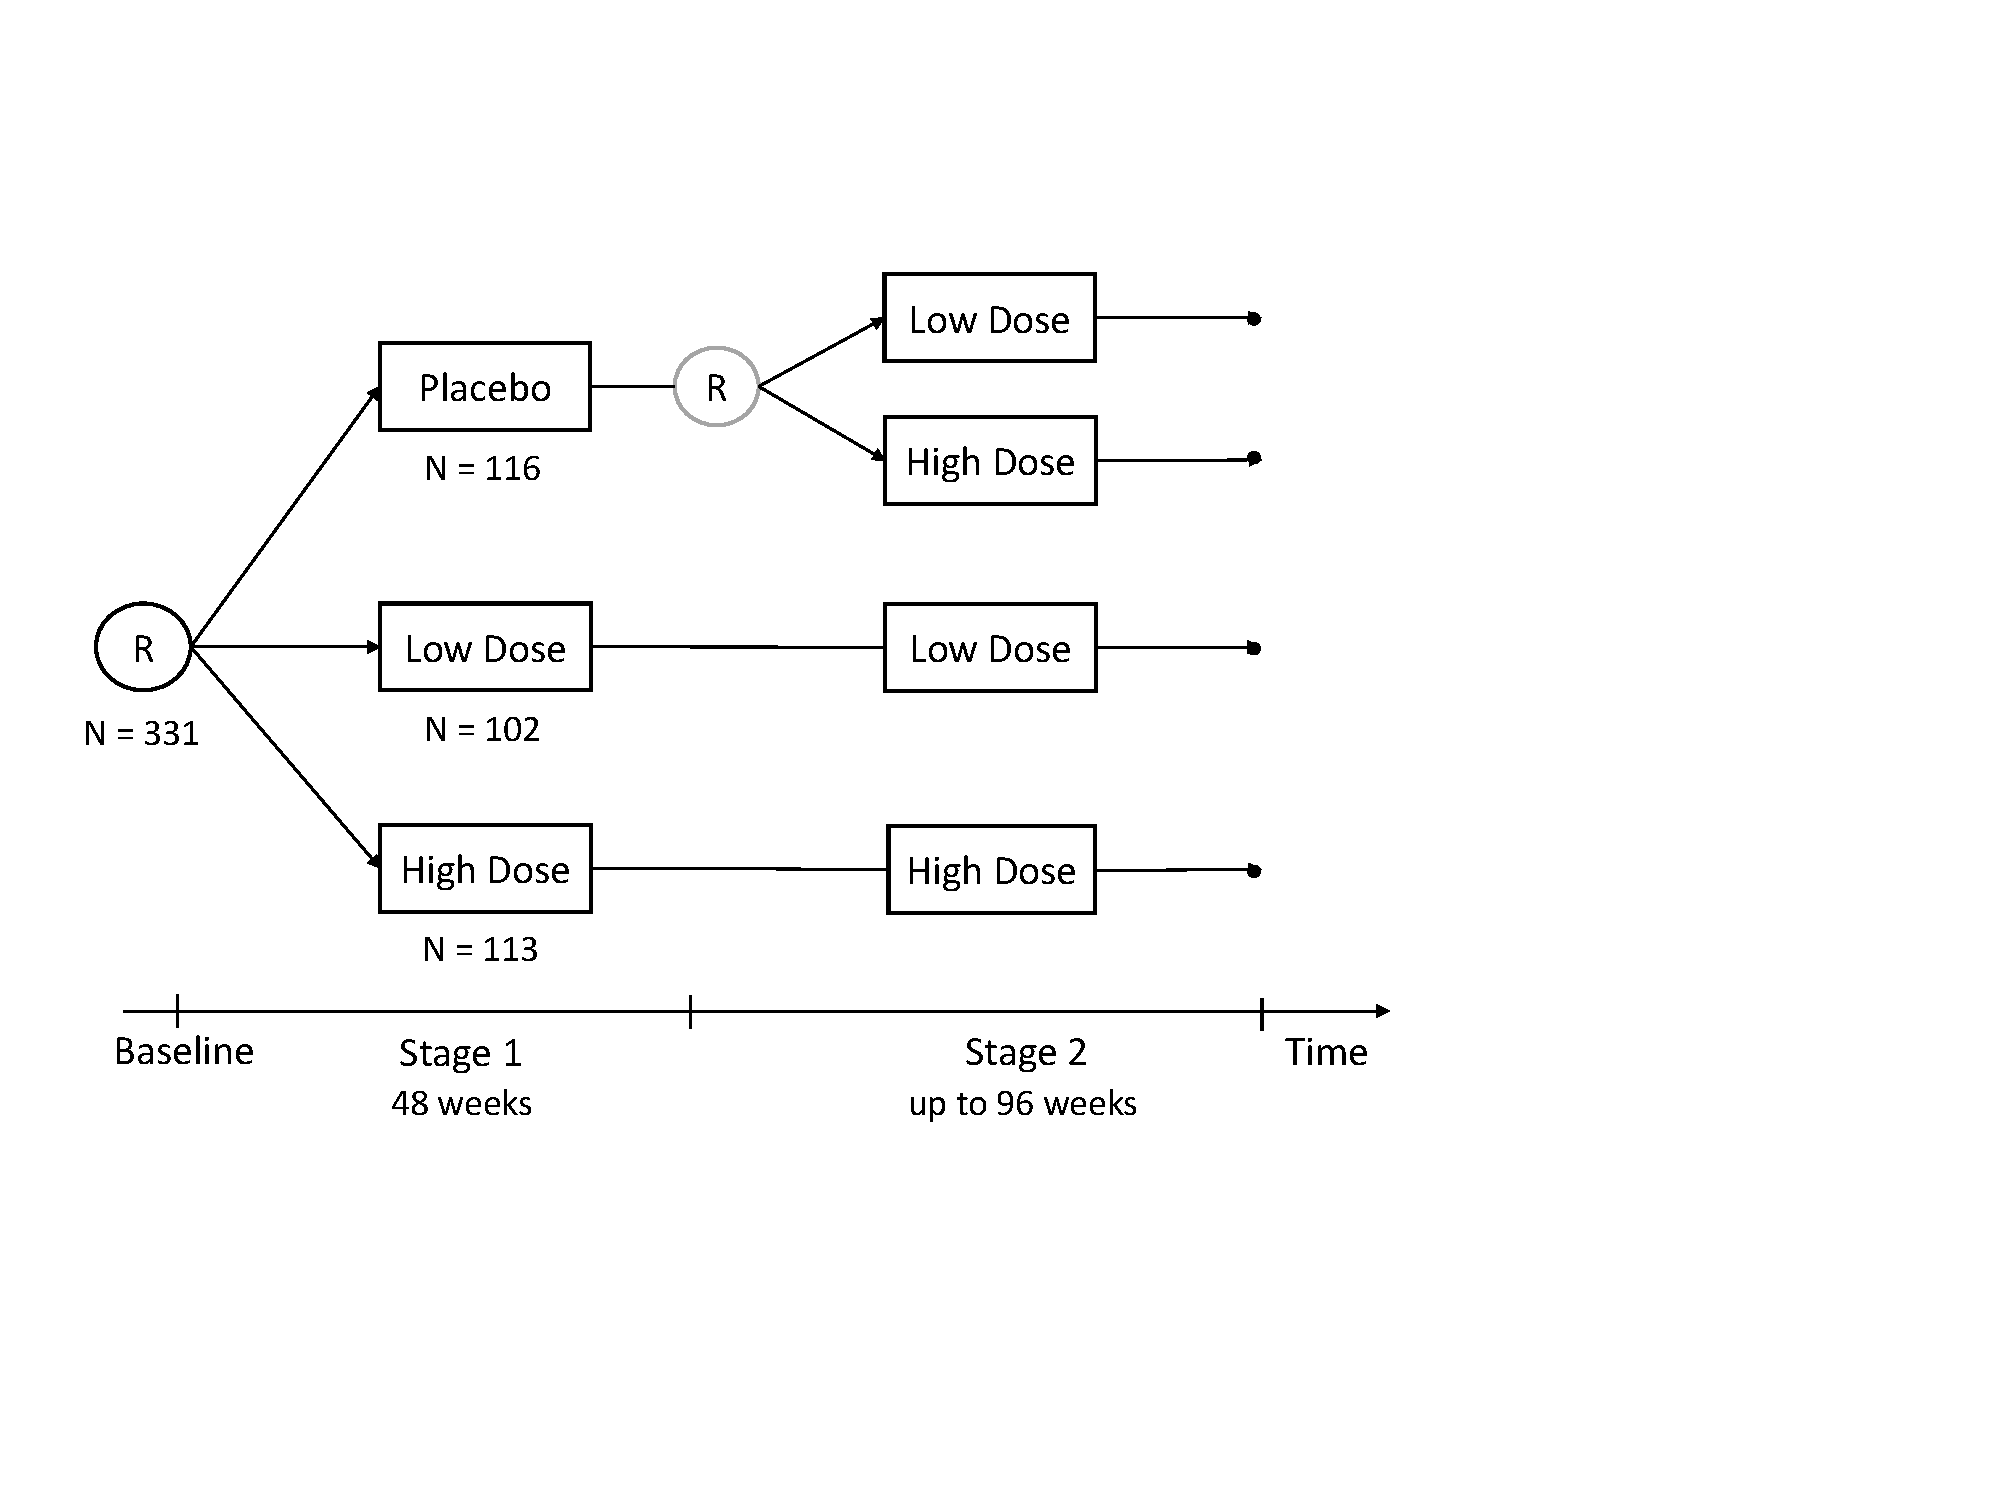
\includegraphics[width=0.7\textwidth]{chapters/figures/tadalafil_design.pdf}\label{fig:tadalafil}}
\\
\subfloat[]{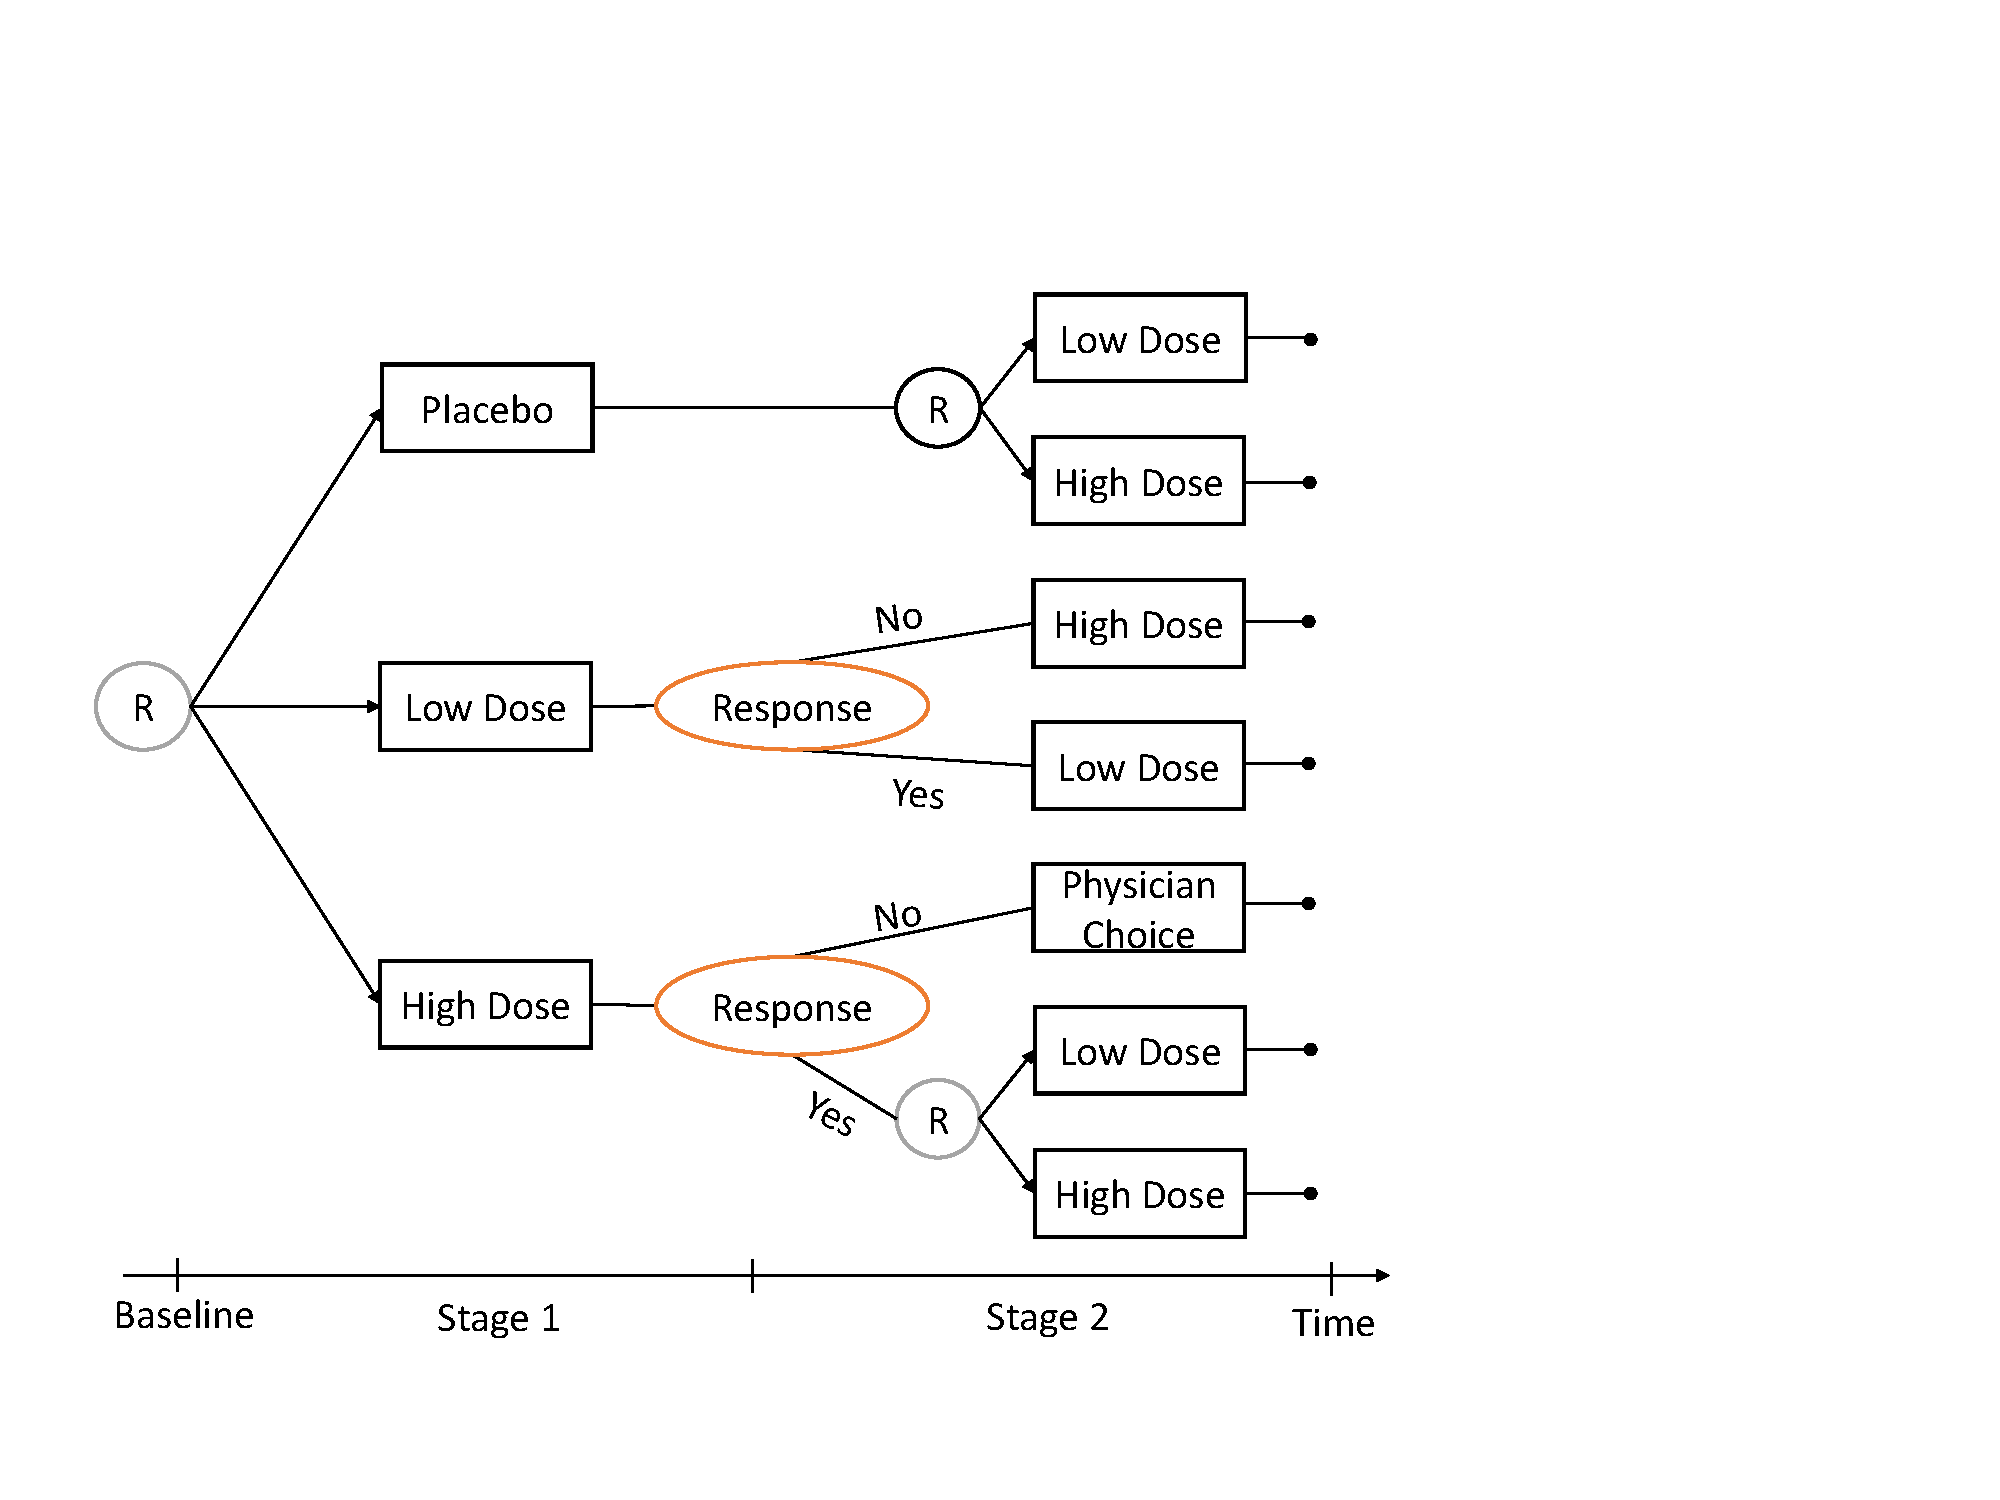
\includegraphics[width=0.7\textwidth]{chapters/figures/snSMART_design_longitudinal.pdf}\label{fig:codatasnSMART_longitudinal}}
\caption{(a) Study design of the tadalafil trial (NCT01865084). (R) denotes randomization. (b) Study design of the snSMART design \citep{wang2023dynamic} that formally incorporates external control data. Participants are randomized (R) with 1:2:2 chances of receiving placebo, low dose, or high dose, respectively, in stage 1. At the end of stage 1, participants are assigned or re-randomized to their stage 2 treatment based on their stage 1 treatment and response status. Outcomes are collected at the end of stage 1 and 2.}
\end{figure}



\subsection{Proposed Modification for Tadalafil Trial Design}

In the \ac{snSMART} design \citep{wang2023dynamic}, illustrated in Figure \ref{fig:codatasnSMART_longitudinal}, patients are initially randomized in a 1:2:2 ratio to receive either a placebo, a low dose, or a high dose (e.g., of tadalafil) in stage 1. After 48 weeks, participants are re-assigned or re-randomized based on their initial treatment and post-baseline 6MWD. According to the protocol of the tadalafil trial, a participant is considered a responder at week 48 if their post-baseline \ac{6MWD} does not decrease by more than 10\%. Those who received a placebo in stage 1 are equally re-randomized to either a low or high dose in stage 2, independent of their stage 1 response, ensuring all participants receive treatment. For participants initially on a low dose, responders remain on it, while non-responders switch to a high dose. High dose responders in stage 1 are equally re-randomized to either low or high dose, considering the potential efficacy and tolerability of a lower dose. However, non-responders to the high dose are excluded from stage 2 to avoid unnecessary toxicity and ethical concerns, as a lower dose is unlikely to be effective if a higher dose proved ineffective. This design choice aims to optimize treatment effectiveness and ethical considerations in the trial.

\section{Methods}
\label{sec:methods}

\subsection{Mixed Model Repeated Measures (MMRM)}
Traditionally, longitudinal data are most commonly analyzed using a \ac{MMRM} analysis to test the primary null hypothesis of no difference between each treatment (i.e., low and high dose tadalafil) and placebo in mean change in treatment outcomes. The \ac{MMRM} model typically includes a fixed effect for baseline primary outcomes, in our case, 6MWD, as well as fixed effects for treatment group assignment, visit, treatment group-by-visit interaction, and a random effect for subjects. An unstructured covariance matrix is typically used to model the within-subject errors. Note that a traidtional analytiic method does not incoporate external control data and uses only stage 1 outcomes in the analysis.

\subsection{Bayesian joint stage model}

The \ac{snSMART} design can be analyzed with a customized \ac{BJSM}. Unlike the does level \ac{BJSM} proposed by \cite{fang2023comparing}, which uses data from two stages without incorporating external data, our approach involves integrating external control data using informative normal distribution priors for the placebo effect parameter. This involves estimating the prior's parameters through a method of moments approximation from external data and adjusting the variance to reach the desired \ac{ESS}.

\subsection{Bayesian longitudinal piecewise meta-analytic combined (BLPM) approaches}
The primary analysis using our proposed \ac{BLPM} approach involves a two-step procedure: 1) calculating the \ac{PS} \citep{rosenbaum1983central} for all external control patients by fitting a logistic regression model to patients in both external controls and the current trial, and 2) fitting the \ac{BLPM} model to both external controls and all current trial data to estimate the treatment effects. The structure of the \ac{BLPM} approach is illustrated in Figure \ref{fig:BLPM_diagram}. More details on each step will be provided in the following sections.


\subsubsection{Notations}
The following notation is used in this section. $Y_{d(i)jk}$ and $\mu_{d(i)jk}$ denote the observed and underlying true outcome (e.g., \ac{NSAA} score or \ac{6MWD}) for patient $i$ at visit $j = 1,...,n_j$ in stage $k = 1, 2$ of trial $d = 1,...,n_d,\star$. Here, we use $d = \star$ to denote current trial, and use $d = 1,...,n_d$ to denote the $n_d$ external controls we collected. We use $l$ and $h$ to denote low dose and high dose, respectively. Thus, $Y_{\star(10)31}$ denotes the observed outcome of current trial patient 10 at third visit in stage 1, and $Y_{3(1)41}$ denotes the observed outcome of patient 1 in the 3rd external control data at fourth visit in stage 1. We use $\boldsymbol{X}$ or $\boldsymbol{Z}$ to denote the baseline covariate matrix, and use $\beta$s and $b$s to denote the fixed effect coefficients and random effects, respectively. $T_{1i}$ and $T_{2i}$ are used to denote stage 1 treatment and stage 2 treatment received by subject $i$ in current trial $\star$. $\omega$s stands for the \ac{IPTW} of subjects.

\begin{figure}
\centering
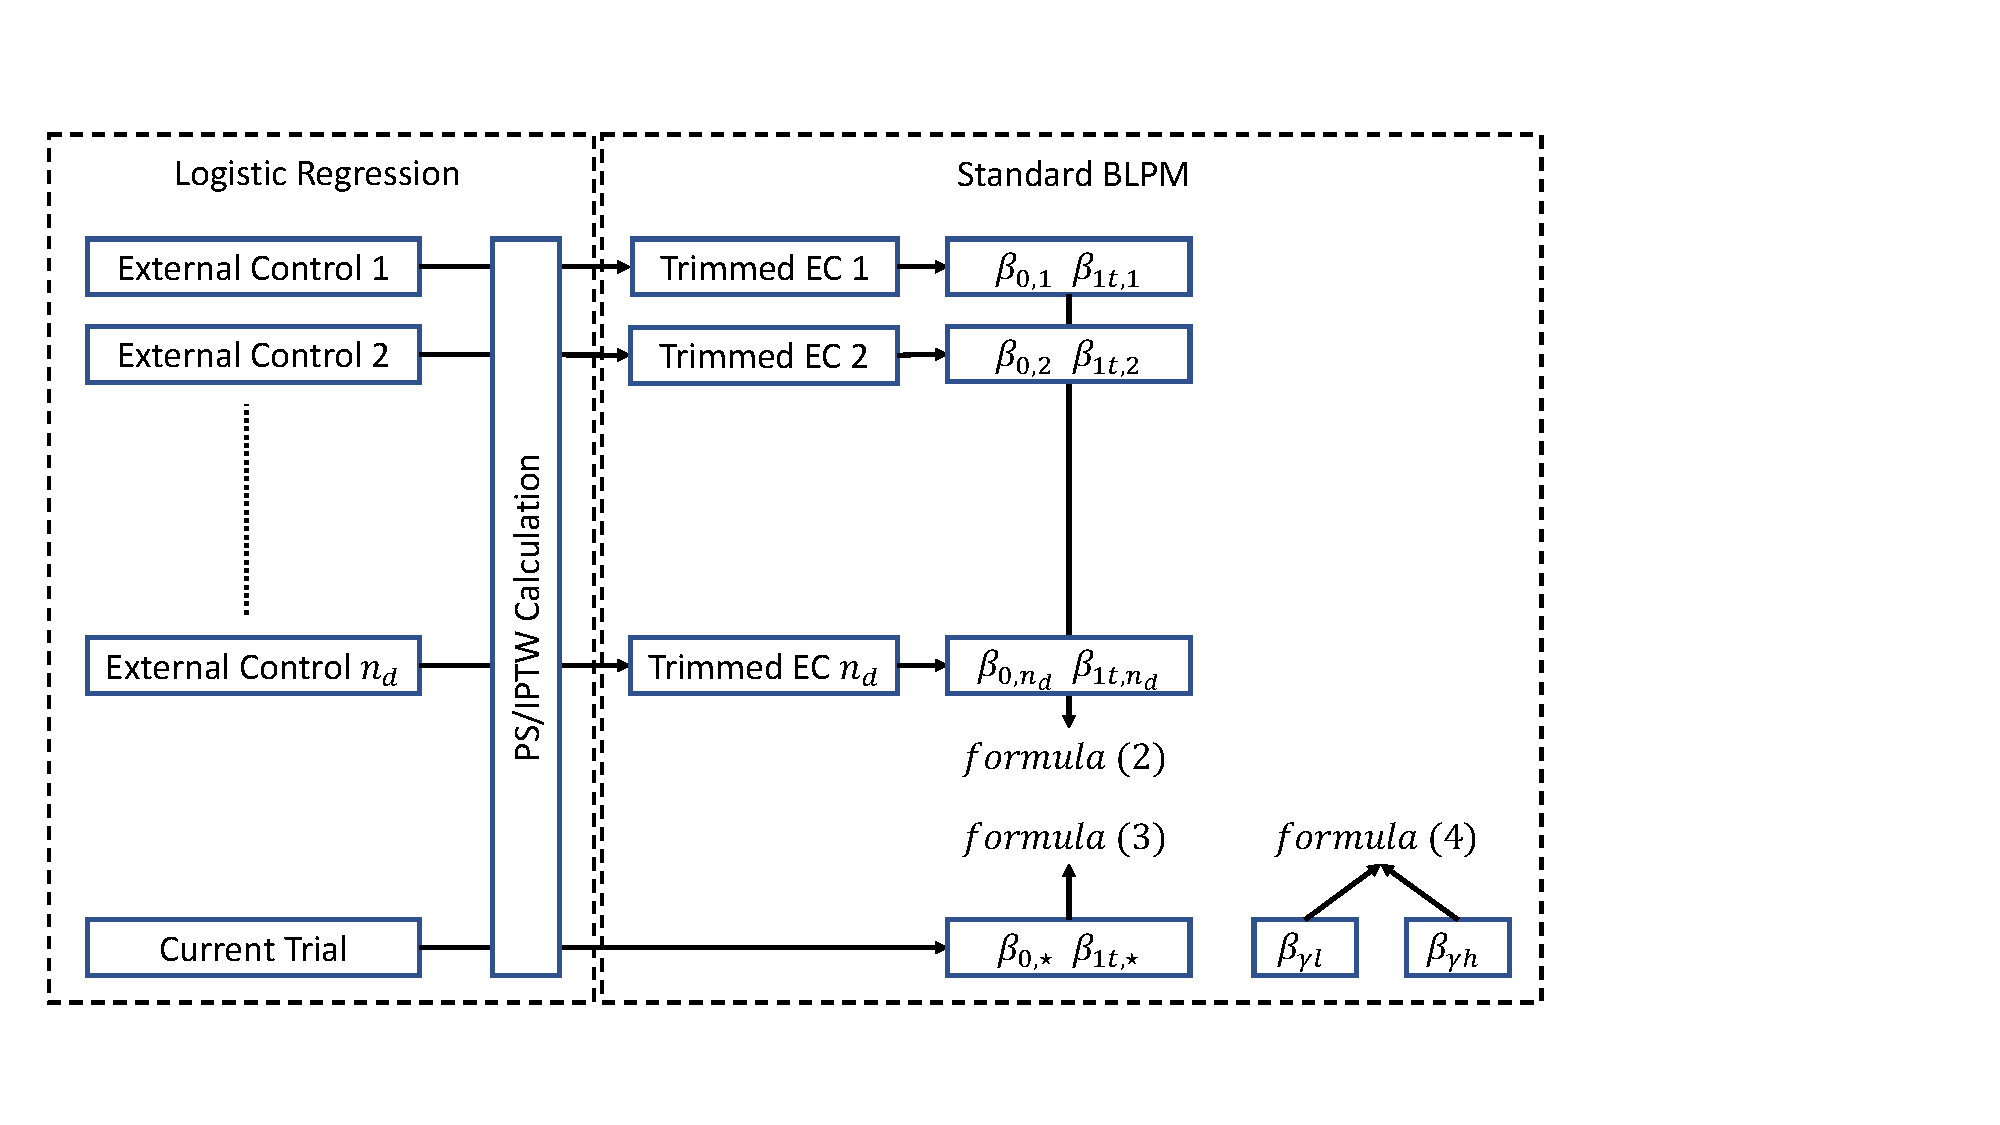
\includegraphics[width=\textwidth]{chapters/figures/flow.pdf}
\caption{Structure of the standard BLPM approach}
\label{fig:BLPM_diagram}
\end{figure}

\subsubsection{PS and IPTW calculation} \label{sec:ps}

Controlling for potential bias is essential when using external control data in clinical trials. To combat bias, especially from unmeasured confounders, it's important to prespecify statistical methods. Addressing measured confounders starts with carefully selecting external control data. \cite{pocock1976combination} and \cite{lim2018minimizing} have outlined criteria for assessing the similarity between external and trial control data. 

In our context, after excluding subjects from the external controls who do not meet the inclusion and exclusion criteria of the current trial, and after collecting all baseline covariates for those retained in the external controls and those enrolled in the current trial, the \ac{PS} can be calculated. The \ac{PS} is defined as the probability of a subject being from the current study rather than from external data sources. The logistic regression used to obtain the \ac{PS} estimates can be formulated as: $StudyIndicator_{di} = \boldsymbol{X}_{di}\boldsymbol{\beta} + \epsilon_{di}$, where $StudyIndicator_{\star i} = 1$ if the patient is from the current trial, and $StudyIndicator_{di} = 0$ if patient $i$ is from one of the external control datasets $d$. Specifically for the tadalafil trial, covariates may include variables such as \textit{age}, \textit{race}, \textit{ethnicity}, \textit{height}, \textit{weight}, \textit{baseline NSAA} and \textit{baseline 6MWD}.

The \ac{IPTW} for participants is determined using the stabilized weighting method, which facilitates the calculation of the average treatment effect in the treated (ATT). In this approach, subjects from the current trial are assigned a weight of 1 to maximize the utilization of the current trial data. For subjects in the external control group, weights are computed using the formula $\omega_{di}' = PS_{di} / (1 - PS_{di})$, and then normalized to $\omega_{di} = \omega_{di}' / (\sum_{i \in trial\, d} \omega_{di}' / N_{d})$, where $N_d$ represents the total number of subjects in trial $d$.

Next, we trim the external controls to retain only those subjects whose \ac{PS} fall within the range of the \ac{PS} of all subjects in the current trial. This step further reduces heterogeneities between data sources. However, despite careful selection and \ac{PS} trimming, clinical outcomes may vary across sources due to various intrinsic and extrinsic factors, necessitating a model-based approach for proper analysis.

\subsubsection{Structure the Bayesian longitudinal piecewise model across trial stages}

Given the relatively stable rate of decrease in observed \ac{6MWD} and \ac{NSAA} over time in the tadalafil trial \citep{victor2017phase}, we adopt a piecewise linear regression model \citep{nahum2020smart}. This model fits a separate line segment for different trial stages, allowing the linear trend in the outcome during stage 1 to differ from that during stage 2. If the rate of decrease varies significantly between visits, shorter time intervals for each line segment can be applied. Under the proposed \ac{snSMART} design, a subject in the current trial could follow one of seven distinct treatment sequences: ($p$ then $l$), ($p$ then $h$), ($l$ then $l$), ($l$ then $h$), ($h$ then $l$), ($h$ then $h$), and ($h$ with \textit{No stage 2 treatment}). In contrast, a subject in the external controls can be considered as being in the placebo arm in stage 1 only. Consequently, our piecewise linear model for both current trial and external control subjects can be formulated as follows:
$$Y_{d(i)jk} \sim N(\mu_{d(i)jk}, \sigma_{d}^2/\omega_{di}),$$
\begin{equation}
\begin{split}
    \mu_{d(i)jk} = & \beta_{0,d} + \beta_{1t,d} \times t_d + b_{1i,d} + b_{2i,d} \times t_d + \boldsymbol{Z}_{i,d}\boldsymbol{\beta}_{z,d} + (\beta_{1l} I[T_{1di}=l] + \beta_{1h} I[T_{1di}=h]) \times t_1  + \\
    & (\beta_{2l1} I[T_{1di}=p, T_{2di}=l] + \beta_{2h1} I[T_{1i}=p, T_{2i}=h] + \beta_{2l2} I[T_{1i}=l, T_{2i}=l] + \\
    & \beta_{2h2} I[T_{1i}=l, T_{2i}=h] + \beta_{2l3}I[T_{1i} = h, T_{2i} = l] + \beta_{2h3} I[T_{1i}=h, T_{2i}=h])\times t_2,
\end{split}
\label{eqn:bwlp}
\end{equation}
where $\boldsymbol{Z}$ is the baseline covariates, $\omega_{di}$, introduced previously in Section \ref{sec:ps}, is included to further reduce the impact of external control subjects who are dissimilar to those in the current trial. \(\beta_{0, d}\) and \(\beta_{1t,d}\) are trial-specific and represent the model intercept and the natural \ac{DMD} disease progression time (placebo) effect, respectively. \(\beta_{1l}\), and \(\beta_{1h}\) represent the treatment effect difference between stage 1 low dose and the time (placebo) effect, and the treatment effect difference between stage 1 high dose and the time (placebo) effect, respectively. Similarly, \(\beta_{2l1}\) denotes the treatment effect difference between stage 2 low dose and the time (placebo) effect when the subject received placebo in stage 1, \(\beta_{2h1}\) denotes the treatment effect difference between stage 2 high dose and the time (placebo) effect when the subject received placebo in stage 1, \(\beta_{2l2}\) denotes the treatment effect difference between stage 2 low dose and the time (placebo) effect when the subject received low dose in stage 1, and so on. The key estimands of interest are the stage 1 differences in treatment effects between each dose and placebo ($\beta_{1l}$, $\beta_{1h}$). In this model, \( t_{\star} = t_1 + t_2 \), where \( t_1 = 1, \ldots, n_j \) and \( t_2 = 0, \ldots, n_j \). For example, when an observation gathered at stage 1 visit 1 is fitted, \( t_1 = 1 \), \( t_2 = 0 \), and \( t_{\star} = 1 \); similarly, when observations gathered at stage 2 visit 2 are fitted, \( t_1 = 4 \), \( t_2 = 2 \), and \( t_{\star} = 6 \). To account for between-individual heterogeneity in the model, both a trial-specific subject-level random slope, denoted as $b_{2i, d}$, and a random intercept, $b_{1i, d}$, are included. $(b_{1i, d}, b_{2i, d})$ are zero-mean bivariate Gaussian variables with variances $\sigma_{b1, d}^2$ and $\sigma_{b2, d}^2$ respectively, and a correlation coefficient $\rho_{1,d}$.

\subsubsection{\texorpdfstring{Use of external information for $\beta_{0, \star}$, $\beta_{1t,\star}$, $\sigma_{b1,\star}$ and $\sigma_{b2,\star}$}{Use of external information for certain parameters}} \label{sec:external}
To more effectively utilize the external controls we gathered, we could employ the robust \ac{MAC} approaches, detailed in \cite{neuenschwander2016use} and \cite{wang2023dynamic}, to assist in estimating the coefficients $\beta_{0, \star}$, $\beta_{1t, \star}$, $\sigma_{b1, \star}$, and $\sigma_{b2, \star}$. The robust \ac{MAC} structure for $\beta_{0,\star}$ and $\beta_{1t, \star}$ of current trial and $\beta_{0,d}$ and $\beta_{1t,d}$ of external control $d$ is specified as below:
\begin{equation}\label{eq:BLPM}
\begin{bmatrix} \beta_{0,d} \\ \beta_{1t,d} \end{bmatrix} \sim p_d \times BVN\left(\\ \begin{bmatrix} \mu_{0} \\ \mu_{1}\end{bmatrix}, \boldsymbol{V}(\tau_{0,d}, \tau_{1,d})\right) 
+ (1 - p_d) \times BVN\left(\\ \begin{bmatrix} m_{0,d} \\ m_{1,d}\end{bmatrix}, \boldsymbol{V}(v_{0,d}, v_{1,d})\right),
\end{equation}   

\begin{equation}\label{eq:mac}
\begin{bmatrix} \beta_{0,\star} \\ \beta_{1t,\star} \end{bmatrix} \sim p_\star \times BVN\left(\\ \begin{bmatrix} \mu_{0} \\ \mu_{1}\end{bmatrix}, \boldsymbol{V}(\tau_{0,\star}, \tau_{1,\star})\right) 
+ (1 - p_\star) \times BVN\left(\\ \begin{bmatrix} m_{0,\star} \\ m_{1,\star}\end{bmatrix}, \boldsymbol{V}(v_{0,\star}, v_{1,\star})\right),
\end{equation}   

where $$\boldsymbol{V}(\tau_{0,d}, \tau_{1,d}) = \begin{bmatrix} \tau_{0,d}^2 & \rho_{01\tau,d}\tau_{1,d}\tau_{0,d}\\ \rho_{01\tau,d}\tau_{1,d}\tau_{0,d} & \tau_{1,d}^2\end{bmatrix}, \boldsymbol{V}(v_{0,d}, v_{1,d}) = \begin{bmatrix} v_{0,d}^2 & \rho_{01v,d}v_{1,d}v_{0,d}\\ \rho_{01v,d}v_{1,d}v_{0,d} & v_{1,d}^2\end{bmatrix},$$

$$\boldsymbol{V}(v_{0,\star}, v_{1,\star}) = \begin{bmatrix} v_{0,\star}^2 & \rho_{01,\star}v_{1,\star}v_{0,\star}\\ \rho_{01,\star}v_{1,\star}v_{0,\star} & v_{1,\star}^2\end{bmatrix}.$$

$p_d$ and $p_\star$ determine the resemblance between $\beta_{0,d}$ and $\beta_{1t,d}$ of external control dataset $d$ and current trial $\beta_{0, \star}$ and $\beta_{1t,\star}$. The selection of values for $m_{0,d}, m_{1,d}, m_{0,\star}, m_{1,\star}, v_{0,d}, v_{1,d}, v_{0,\star}$, and $v_{1,\star}$ relies on expert insights. If no expert insights are available, weakly informative priors can be used \citep{kass1995reference}.
In doing so, we further down-weight the non-exchangeable external data based on variability between data sources, aiming to borrow approximately the same amount of information as in the design stage. In addition to $\beta_{0,d}$ and $\beta_{1t,d}$, a similar mixture of bivariate normal distributions can also be used to incorporate external information into the estimation of $\sigma_{b1,\star}$ and $\sigma_{b2,\star}$.

\subsubsection{Combining evidence for low and high dose groups}
Given that our model assumes exchangeable treatment effects across trial stages, and since the original purpose of designing stage 2 of the current trial is to gather more data to assess the treatment effect in stage 1, it is logical to add a component to the method that combines the data from all low dose and high dose groups to achieve better estimation efficiency. Therefore, we assume that 

\begin{equation}
\beta_{\gamma_l} \sim N(\mu_l, \tau_{\gamma_l}^2); \quad \beta_{\gamma_h} \sim N(\mu_h, \tau_{\gamma_h}^2),
\end{equation}
where $\gamma_l = 1l, 2l1, 2l2, 2l3$ and $\gamma_h = 1h, 2h1, 2h2, 2h3$. The \ac{snSMART} design, suitable for stable conditions with a required washout period between stages, supports the assumption of exchangeable treatment effects. If stage-wise non-exchangeability is a concern, the robustification (mixture) component outlined in Section  \ref{sec:external} can be integrated into the distribution of treatment effect $\beta$s to address non-exchangeable treatment effects across trial stages. We name this version of the model as the robust \ac{BLPM} model. In this paper, we implement both the standard \ac{BLPM} method and the robust \ac{BLPM} in simulation studies (Section \ref{sec:simulation_longitudinal}) and the reanalysis of tadalafil trial (Section \ref{sec:reanalysis}).

\subsubsection{Missing data imputation}
\label{sec:missing}
Sometimes, the external controls we have found have missing values due to different visiting schedules from the current trial or have been lost to follow-up because the external control trial was stopped. Although the \ac{BLPM} model code can run smoothly with missing data, we recommend conducting multiple imputations to obtain more convincing estimators when the data is missing completely at random (MCAR) or missing at random (MAR). We perform multiple imputation using a Bayesian linear mixed model (LMM) incorporating fixed effects for the intercept, received treatment, visit, baseline outcomes, and various other baseline covariates. Additionally, this model includes subject-level random effects for visits and random intercepts. 

We generate imputed datasets using the \ac{PPD} technique \citep{gelman2014bayesian}. The \ac{PPD} illustrates the distribution of potential unobserved values derived from the observed values, and it adheres to the following structure:
$$p(y_{pred}|y) = \int{p(y_{pred},\theta|y)d\theta} = \int{p(y_{pred}|\theta,y)p(\theta|y)d\theta} = \int{p(y_{pred}|\theta)p(\theta|y)d\theta},$$
This formulation takes advantage of the conditional independence between the observed data $y$, unobserved data $y_{pred}$, and model parameters $\theta$. The \ac{PPD} can be conceptualized as an averaging of conditional predictions across the posterior distribution of $\theta$. For each sampled $\theta$ from the posterior distribution, a corresponding sample of $y_{pred}$ is acquired.

In total, more than 100 imputed datasets should be generated, and to obtain the final estimators, we should combine all the sampled draws from the \ac{MCMC} run on each imputed dataset \citep{zhou2010note}.

\subsubsection{Prior specification}
We suggest generalizable, weakly informative normal distributions as priors for all the $\mu$ parameters, i.e., priors that are worth approximately one observation \citep{kass1995reference}. We suggest using non-informative $Unif(-1,1)$ prior distributions for all the correlation parameters ($\rho$).

Half-normal priors with standard deviations roughly equal to half of the standard deviation of the estimated parameter, i.e., $\beta_{0,\star}$, $\beta_{1t, \star}$, $\sigma_{b1, \star}$ and $\sigma_{b2, \star}$, are recommended for all the $\tau$s, aiming to cover very small to large between-trial heterogeneity. More details about how to specify prior for $\tau$ can be found in \cite{spiegelhalter2004bayesian} and \cite{gelman2006prior}. We suggest weakly informative normal distributions for covariates in the $\boldsymbol{\beta}_{z,d}$ vector and $\sigma$ in Formula \ref{eqn:bwlp}. 


\section{Simulation settings}
\label{sec:simulation_longitudinal}
We assess the sensitivity of our proposed \ac{BLPM} and robust \ac{BLPM} methods similarly to the simulation studies conducted by \cite{wang2023dynamic}. The simulation scenarios cover a range of data generating settings, treatment effects, sample sizes, and instances of non-exchangeability between external control and current \ac{snSMART} data. We evaluate two distinct data generation processes: the first adheres to the proposed model, while the second allows for deviations from exchangeability between stages 1 and 2. The first data generation process assumes stage-wise exchangeability: at the subject level, the placebo, low dose, and high dose treatment effects between visits in stage 1 are generated through normal distributions with predetermined mean and standard deviation values. For stage 2, the low dose and high dose treatment effects for subjects between visits are generated using the same distributions as in stage 1. In the second data generation process, treatment effects for stage 1 and stage 2 are not exchangeable. Specifically, the stage 2 low dose and high dose treatment effects are generated using the same normal distributions as stage 1, but with their means set 1 unit higher than those in stage 1. This type of data could occur in an \ac{snSMART} where the washout period between stages 1 and 2 is inadequate or unexpected disease progression is observed. In addition to treatment effects, we also generated subject-level baseline age, baseline outcome, and the time effect on disease progression using normal distributions. To generate longitudinal data at each visit, it is necessary to sum up all the baseline effects, accumulated time effects, and accumulated treatment effects by each visit. In the simulated datasets, 4 visits are included in both stage 1 and stage 2.

Alongside evaluating various data generation processes, we also explore the efficacy of our proposed models across six distinct treatment effect scenarios, particularly in the context of \ac{DMD}. In this setting, a \ac{NSAA} score of 4 serves as the criterion to distinguish responders from nonresponders at the conclusion of stage 1. For this purpose, we define \(\delta_{1p}, \delta_{1l}\), and \(\delta_{1h}\) as the absolute accumulated treatment effects (e.g., \ac{NSAA} score) for placebo, low dose, and high dose, respectively, by the end of stage 1, and \(\delta_{d}\) represents the absolute placebo treatment effect in external control \(d\). Scenario 1 posits the new drug's ineffectiveness (\(\delta_{d} = \delta_{1p} = \delta_{1l} = \delta_{1h} = 0\)). In Scenario 2, effectiveness is attributed solely to the high dose (\(\delta_{d} = \delta_{1p} = \delta_{1l} = 0 < \delta_{1h} = 6\)). Scenario 3 suggests a modest effect for the low dose and a clinically significant effect for the high dose (\(\delta_{d} = \delta_{1p} = 0 < \delta_{1l} = 2 < \delta_{1h} = 6\)). Lastly, Scenario 4 assumes both low and high doses yield clinically meaningful effects (\(\delta_{d} = \delta_{1p} = 0 < \delta_{1l} = 4 < \delta_{1h} = 8\)). We also created two more scenarios to evaluate our model's sensitivity regarding the alignment between external control and current data (scenario 5: \(\delta_d \ne \delta_{1p}\) for some \(d\); scenario 6: \(\delta_d \ne \delta_{1p}\) for all \(d\)). A comprehensive overview of all simulation scenarios is available in Table \ref{tab:simulation_settings}.

\begin{table}
\caption{Simulation parameters and scenarios.\label{tab:simulation_settings}}
\begin{center}
\vspace{-5mm}
\begin{tablenotes}  
    \small
     \textit{$\delta_{d}$ denotes the mean absolute placebo treatment effect (e.g., NSAA score) in external control $d$ at the end of stage 1, where $d = 1,2,...n_d$. $\delta_{Tk}$ is the mean absolute treatment effect of treatment $T$ at the end of stage $k$, where $T = p,l,h, k = 1,2$, $p = $ placebo, $l = $ low dose, and $h = $ high dose. }\\
     \vspace{2.5mm}
\end{tablenotes}
\begin{tabular}{ccc}
  &  Data Generating Process 1 &  Data Generating Process 2 \tabularnewline
\hline
\multirow{3}{4.5em}{Scenario 1} & $\delta_d = \delta_{1p} = 0$, & $\delta_d = \delta_{1p} = 0$,\\
 & $\delta_{1l} = \delta_{2l} = 0$, & $\delta_{1l} = 0$, $\delta_{2l} = 1$, \\
 & $\delta_{1h} = \delta_{2h} = 0$ & $\delta_{1h} = 0$, $\delta_{2h} = 1$\\  
\hline
\multirow{3}{4.5em}{Scenario 2} & $\delta_d = \delta_{1p} = 0$, & $\delta_d = \delta_{1p} = 0$,\\
 & $\delta_{1l} = \delta_{2l} = 0$, & $\delta_{1l} = 0$, $\delta_{2l} = 1$, \\
 & $\delta_{1h} = \delta_{2h} = 6$ & $\delta_{1h} = 6$, $\delta_{2h} = 7$\\  
\hline
\multirow{3}{4.5em}{Scenario 3} & $\delta_d = \delta_{1p} = 0$, & $\delta_d = \delta_{1p} = 0$,\\
 & $\delta_{1l} = \delta_{2l} = 2$, & $\delta_{1l} = 2$, $\delta_{2l} = 3$, \\
 & $\delta_{1h} = \delta_{2h} = 6$ & $\delta_{1h} = 6$, $\delta_{2h} = 7$\\  
\hline
\multirow{3}{4.5em}{Scenario 4} & $\delta_d = \delta_{1p} = 0$, & $\delta_d = \delta_{1p} = 0$,\\
 & $\delta_{1l} = \delta_{2l} = 4$, & $\delta_{1l} = 4$, $\delta_{2l} = 5$, \\
 & $\delta_{1h} = \delta_{2h} = 8$ & $\delta_{1h} = 8$, $\delta_{2h} = 9$\\  
\hline
\multirow{5}{4.5em}{Scenario 5} & $\delta_d = 1\, or\, 0$, & $\delta_d = 1\, or\, 0$, \\
& $\delta_{1p} = 0$, & $\delta_{1p} = 0$,\\
 & $\delta_{1l} = \delta_{2l} = 4$, & $\delta_{1l} = 4$, $\delta_{2l} = 5$, \\
 & $\delta_{1h} = \delta_{2h} = 8$ & $\delta_{1h} = 8$, $\delta_{2h} = 9$\\ 
\hline
\multirow{3}{4.5em}{Scenario 6} & $\delta_d = 1$, $\delta_{1p} = 0$, & $\delta_d = 1$, $\delta_{1p} = 0$,\\
 & $\delta_{1l} = \delta_{2l} = 4$, & $\delta_{1l} = 4$, $\delta_{2l} = 5$, \\
 & $\delta_{1h} = \delta_{2h} = 8$ & $\delta_{1h} = 8$, $\delta_{2h} = 9$\\ 
\hline
\end{tabular}
\end{center}
\end{table}

Under each data generating process, 1,000 realizations per scenario were simulated. Each realization includes one external control data set and one current \ac{snSMART} data set. Estimations from the \ac{BLPM}, robust \ac{BLPM}, traditional \ac{MMRM} analysis, and \ac{BJSM} are compared. We calculate \ac{CR}, \ac{rMSE}, average bias, and average width of the 95\% \ac{CI} of each estimator. Note that the Monte Carlo error for all average bias and \ac{CI} width is less than 0.005. Finally, type I error (under scenario 1) and power (under scenarios 3-6) of different methods are also calculated using the probability that the 95\% credible intervals of $\hat{\beta}_{1l}$ and $\hat{\beta}_{1h}$ do not include 0. Results are provided for sample size of 25, 50 and 250 randomized with a 1:2:2 ratio to the placebo, low dose, and high dose arms respectively. All computations are done via the R function \texttt{jags} in R package \texttt{rjags} \citep{rjags}.

\subsection{Results}
In data generation process 1, which satisfies stage-wise exchangeability, the left columns of Figure \ref{fig:rMSE_longitudinal}, as well as Figures \ref{fig:Bias_longitudinal}, \ref{fig:CR_longitudinal}, and \ref{fig:Width_longitudinal}, display the \ac{rMSE}, average bias, \ac{CR}, and average \ac{CI} width for $\hat{\beta}_{1l}$ and $\hat{\beta}_{1h}$. Compared to \ac{MMRM} and \ac{BJSM} , estimators from the \ac{BLPM} methods exhibit notably lower rMSEs. The \ac{BLPM} methods achieve similar coverage rates to traditional methods, with a slightly lower \ac{CR} than \ac{MMRM} at $n = 50$ and a slightly higher \ac{CR} when $n = 25$, while offering significantly narrower 95\% \ac{CI} widths in all scenarios. Despite the \ac{BLPM} methods displaying marginally increased average biases in scenario 6, due to completely non-exchangeable external controls, these biases are still negligible.

\begin{figure}
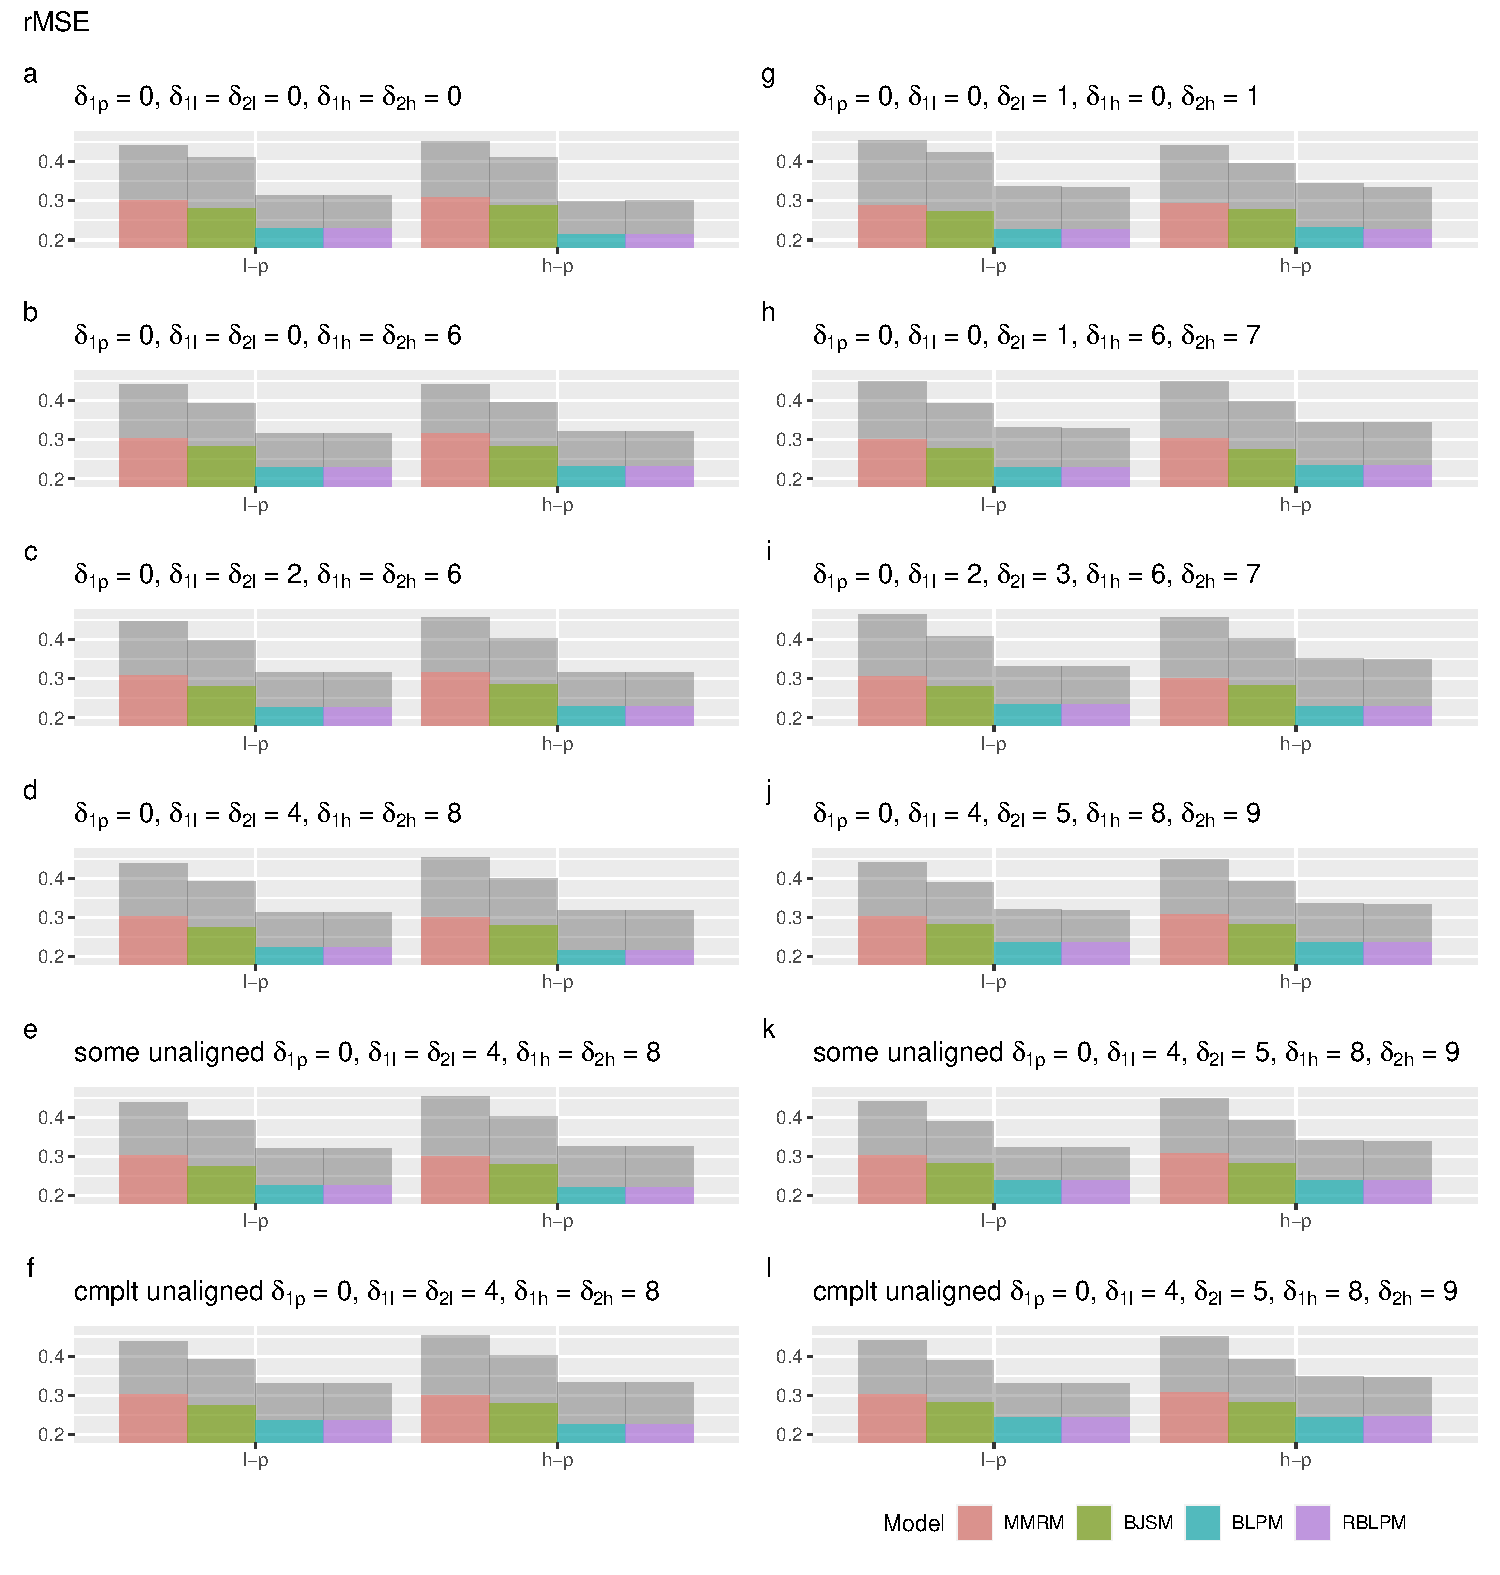
\includegraphics[width=0.95\textwidth]{chapters/figures/rMSE_longitudinal.pdf}
\caption{Simulated root-mean-square error (rMSE) for the estimators of $\beta_{1l}$ and $\beta_{1h}$. \protect \linebreak Note: $\beta_{1l}$ ($\beta_{1h}$) is the treatment effect difference between stage 1 low (high) dose and placebo. Two hierarchical models: \ac{BLPM} and robust \ac{BLPM} (RBLPM) are compared against the traditional MMRM method and the Bayesian Joint Stage Model (BJSM). The results of total sample size 50 are shown as the colored bars, while the results of total sample size 25 are shown as the overlaying grey bars. The simulation settings are described on the top of each graph, where $\delta_{Tk}$ denotes the true value of the expected treatment effects of treatment $T$ in stage $k$, $T = p, l, h$, $k = 1, 2$, and \emph{some/cmplt unaligned} means some/all of the placebo treatment effects in external control data are inconsistent with the placebo treatment effect in the current trial. Monte Carlo error (MCE) is smaller than 0.005 for all estimators. This figure appears in color in the electronic version of this article, and color refers to that version.}
\label{fig:rMSE_longitudinal}
\end{figure}


\begin{figure}
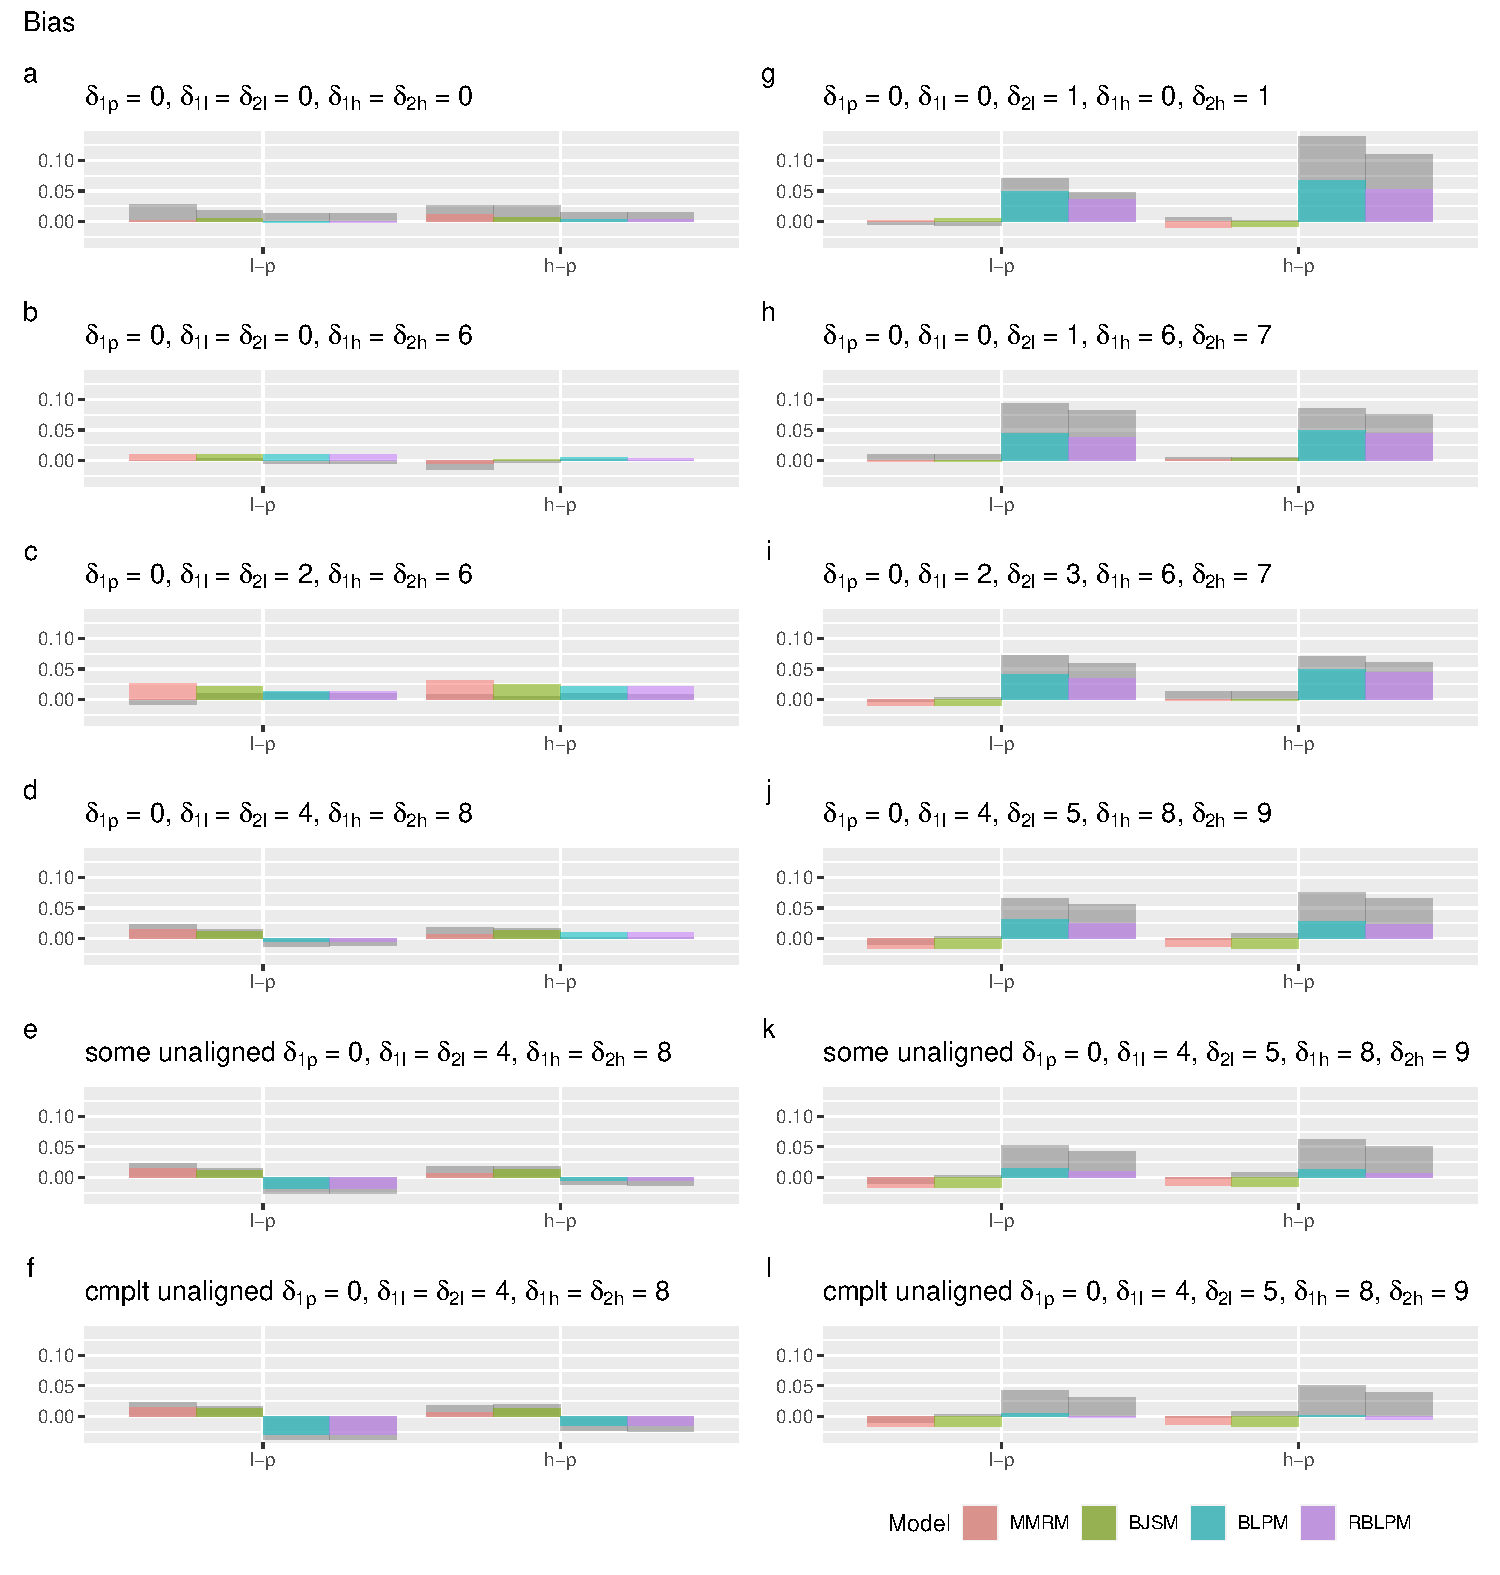
\includegraphics[width=0.95\textwidth]{chapters/figures/Bias_longitudinal.pdf}
\caption{Simulated bias for the estimators of $\beta_{1l}$ and $\beta_{1h}$\\$\beta_{1l}$ ($\beta_{1h}$) is the treatment effect difference between stage 1 low (high) dose and placebo. Two hierarchical models: BLPM and robust BLPM (RBLPM) are compared against the traditional MMRM method and the Bayesian Joint Stage Model (BJSM). The results of total sample size 50 are shown as the colored bars, while the results of total sample size 25 are shown as the overlaying grey bars. The simulation settings are described on the top of each graph, where $\delta_{Tk}$ denotes the true value of the expected treatment effects of treatment $T$ in stage $k$, $T = p, l, h$, $k = 1, 2$, and \emph{some/cmplt unaligned} means some/all of the placebo treatment effects in external control data are inconsistent with the placebo treatment effect in the current trial. Monte Carlo error (MCE) is smaller than 0.005 for all estimators.}
\label{fig:Bias_longitudinal}
\end{figure}


\begin{figure}
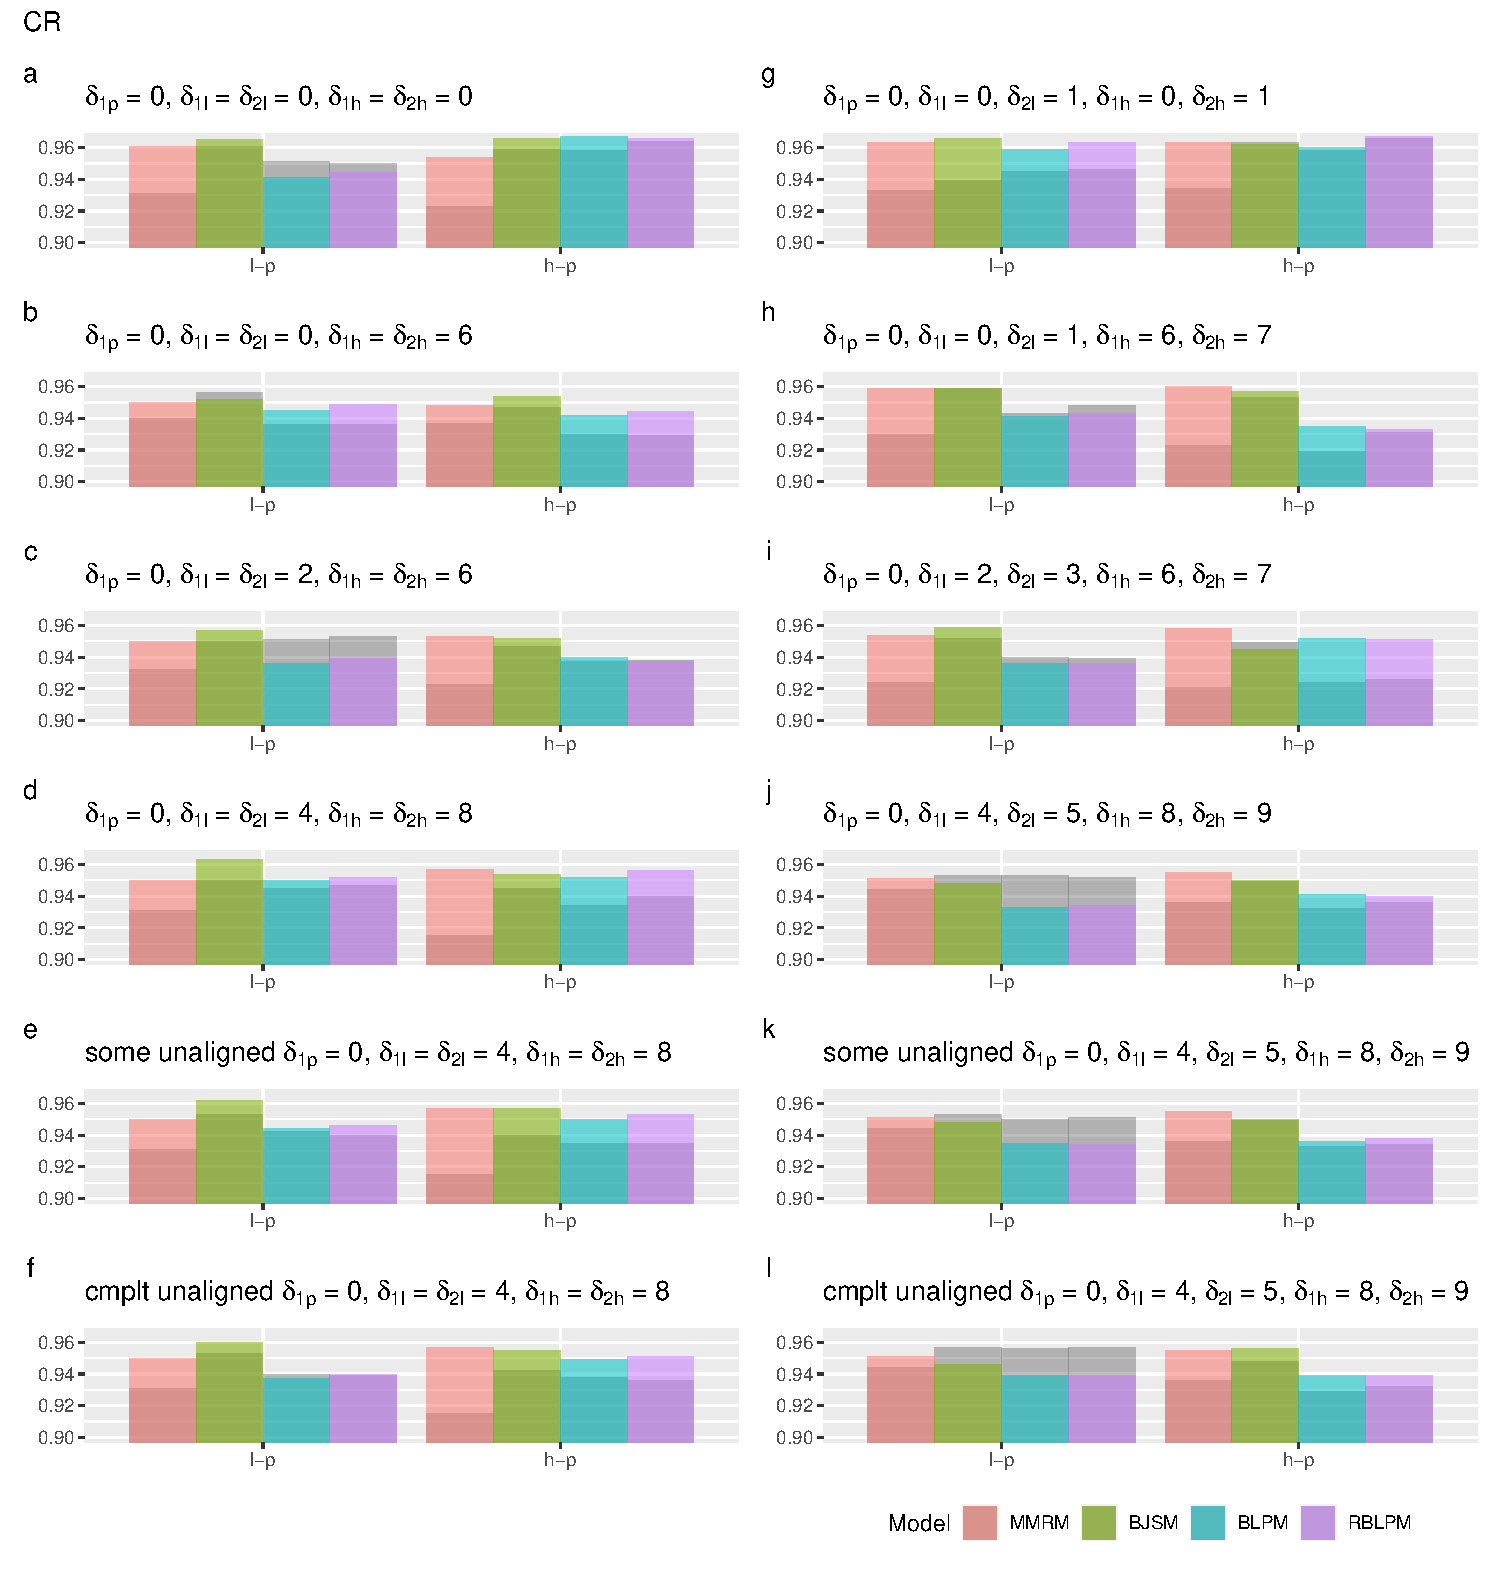
\includegraphics[width=0.95\textwidth]{chapters/figures/CR_longitudinal.pdf}
\caption{Simulated 95\% coverage rate (CR) for the estimators of $\beta_{1l}$ and $\beta_{1h}$\label{fig:CR_longitudinal}\\$\beta_{1l}$ ($\beta_{1h}$) is the treatment effect difference between stage 1 low (high) dose and placebo. Two hierarchical models: BLPM and robust BLPM (RBLPM) are compared against the traditional MMRM method and the Bayesian Joint Stage Model (BJSM). The results of total sample size 50 are shown as the colored bars, while the results of total sample size 25 are shown as the overlaying grey bars. The simulation settings are described on the top of each graph, where $\delta_{Tk}$ denotes the true value of the expected treatment effects of treatment $T$ in stage $k$, $T = p, l, h$, $k = 1, 2$, and \emph{some/cmplt unaligned} means some/all of the placebo treatment effects in external control data are inconsistent with the placebo treatment effect in the current trial. Monte Carlo error (MCE) is smaller than 0.005 for all estimators.}
\end{figure}


\begin{figure}
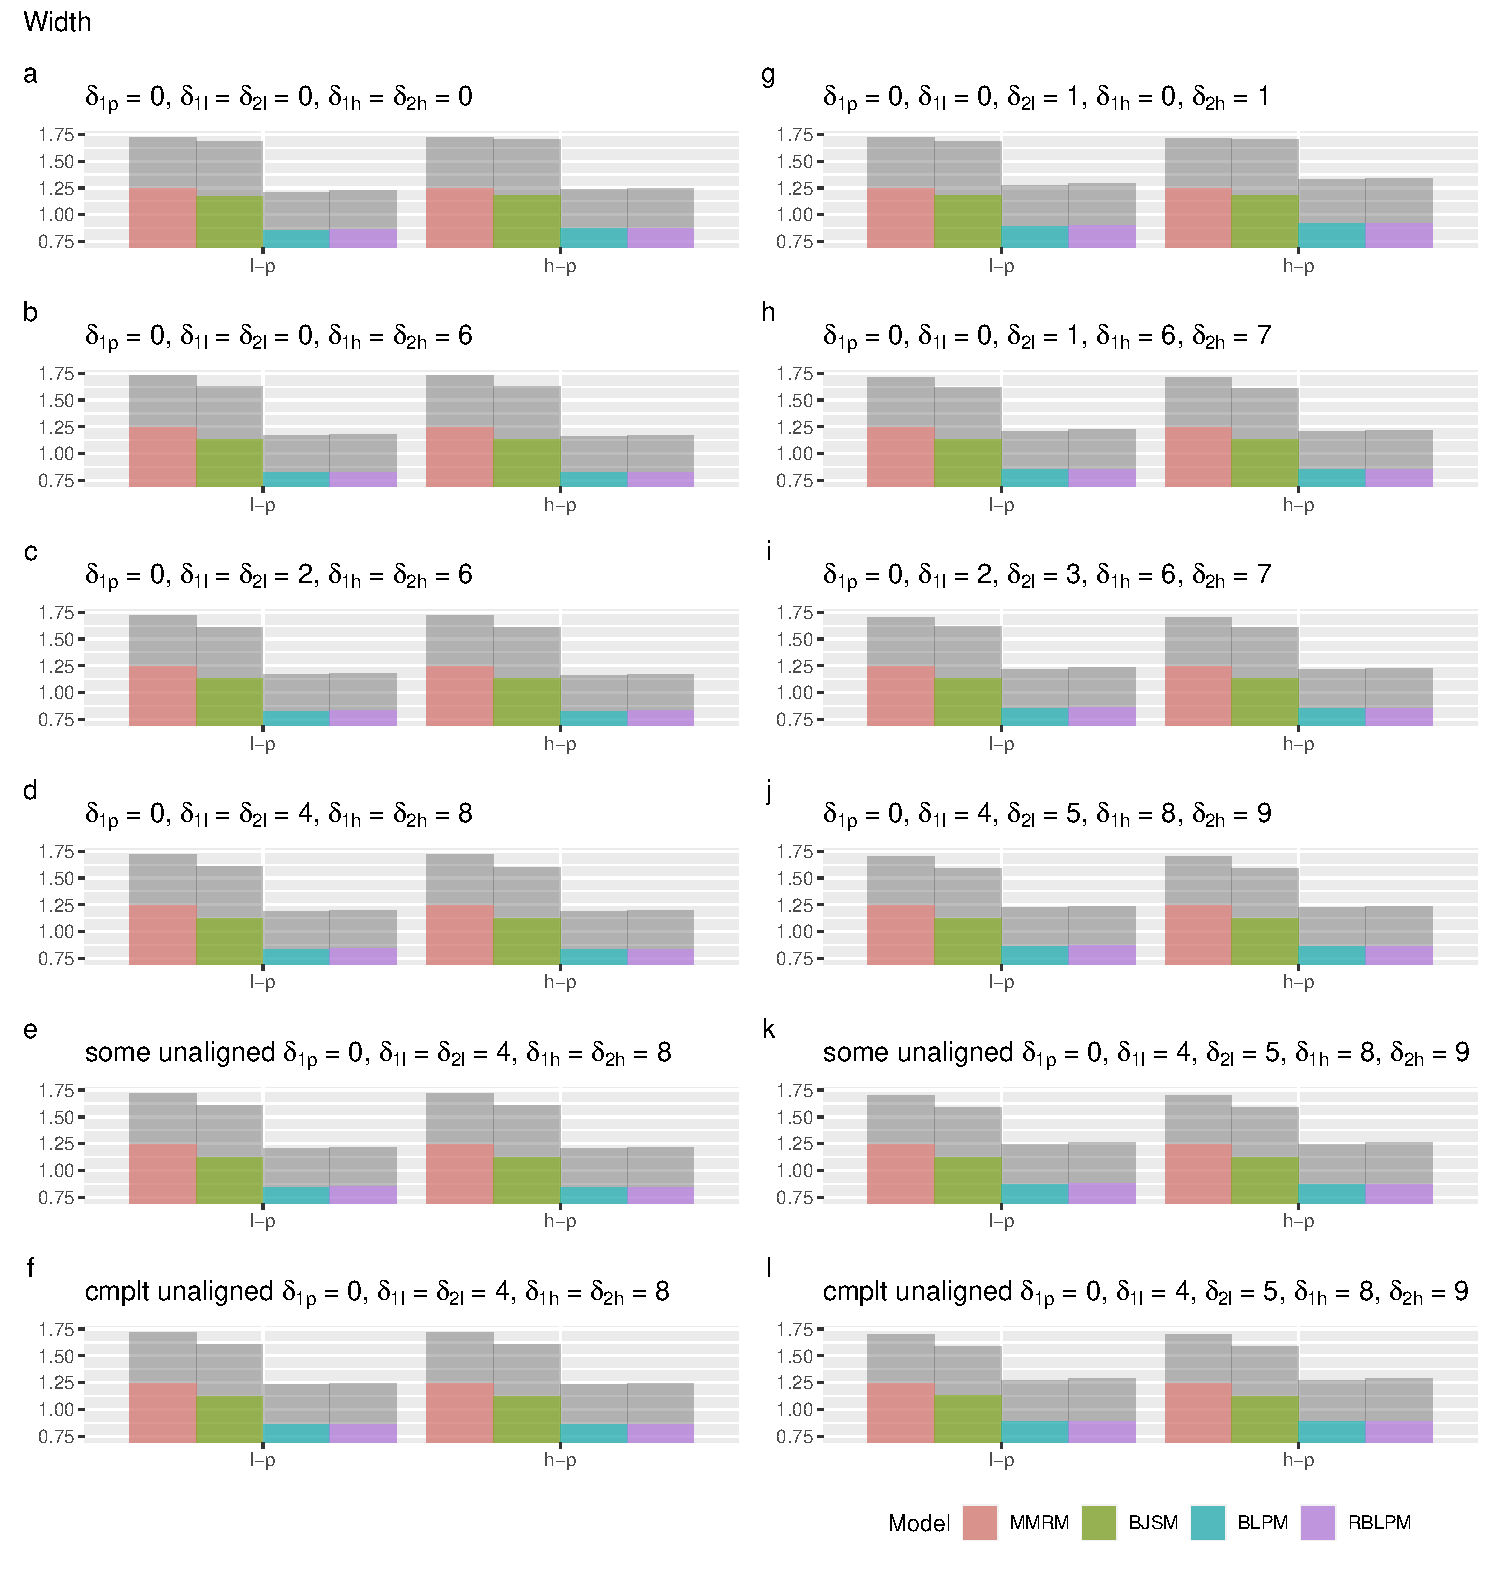
\includegraphics[width=0.95\textwidth]{chapters/figures/Width_longitudinal.pdf}
\caption{Simulated width for the estimators of $\beta_{1l}$ and $\beta_{1h}$\label{fig:Width_longitudinal}\\$\beta_{1l}$ ($\beta_{1h}$) is the treatment effect difference between stage 1 low (high) dose and placebo. Two hierarchical models: BLPM and robust BLPM (RBLPM) are compared against the traditional MMRM method and the Bayesian Joint Stage Model (BJSM). The results of total sample size 50 are shown as the colored bars, while the results of total sample size 25 are shown as the overlaying grey bars. The simulation settings are described on the top of each graph, where $\delta_{Tk}$ denotes the true value of the expected treatment effects of treatment $T$ in stage $k$, $T = p, l, h$, $k = 1, 2$, and \emph{some/cmplt unaligned} means some/all of the placebo treatment effects in external control data are inconsistent with the placebo treatment effect in the current trial. Monte Carlo error (MCE) is smaller than 0.005 for all estimators.}
\end{figure}

\begin{table} 
\caption{\label{tab:TypeI_longitudinal} \centering Simulated type I error. \protect \linebreak
\small
\textit{The type I error of all presented methods is defined as the probability that the credible intervals of $\widehat{\beta}_{1l}$ and $\widehat{\beta}_{1h}$ do not include 0 when there are no treatment effect differences between low dose and placebo and high dose and placebo. Data generating process 1 generates data sets under the assumption that the expected treatment effect of the same dose level is exchangeable across trial stages, and data generating process 2 generates data stage-wise non-exchangeability. $N$ denotes the total number of participants in the trial. Two hierarchical models: standard \ac{BLPM} (BLPM) and robust \ac{BLPM} (RBLPM) are compared against the traditional MMRM and the Bayesian Joint Stage Model (BJSM)}}
\centering
\begin{tabular}{ccccccccc}
\hline
\centering \multirow{2}{*}{Sample Size} & \multicolumn{2}{c}{MMRM} & \multicolumn{2}{c}{BJSM} & \multicolumn{2}{c}{BLPM} & \multicolumn{2}{c}{RBLPM}\\
\centering  & Low & High & Low & High & Low & High & Low & High \\
\hline
\multicolumn{3}{l}{\textit{Data generating process 1}} &&&& \\
$N = 250$ & 0.070 & 0.059  & 0.032 & 0.028 & 0.039 & 0.018 & 0.042 & 0.022 \\
$N = 50$ & 0.04 & 0.05  & 0.04 & 0.03 & 0.06 & 0.04 & 0.06 & 0.04 \\
$N = 25$ & 0.07 & 0.08 & 0.04 & 0.04 & 0.06 & 0.05 & 0.06 & 0.05 \\

\multicolumn{3}{l}{\textit{Data generating process 2}} &&&& \\
$N = 250$ & 0.057 & 0.059 & 0.031 & 0.026 & 0.061 & 0.056 & 0.065 & 0.060 \\
$N = 50$ & 0.04 & 0.04 & 0.04 & 0.04 & 0.05 & 0.05 & 0.05 & 0.04 \\
$N = 25$ & 0.07 & 0.07 & 0.06 & 0.04 & 0.06 & 0.05 & 0.05 & 0.04\\
\hline
\end{tabular}
\end{table}

A comparison across all metrics between the traditional method, \ac{BJSM} , and the \ac{BLPM} methods demonstrates the superior efficiency and accuracy of the \ac{BLPM} methods. Incorporating external control data and stage 2 data from the current trial significantly enhances the estimation of treatment effects. The \ac{BLPM} models adeptly manage the heterogeneity between external controls and current trial data, as evidenced by the minimal increase in rMSEs and average biases in Scenarios 5 and 6 compared to Scenario 4. This confirms the effectiveness of \ac{PS} trimming, \ac{IPTW} weighting, and the \ac{MAC} borrowing structure in addressing discrepancies between data sources, ensuring that the borrowing of external controls remains prudent, even when external controls are completely misaligned with the data from the current trial.


The right columns of Figure \ref{fig:rMSE}, \ref{fig:Bias_longitudinal}, \ref{fig:CR_longitudinal}, and \ref{fig:Width_longitudinal} reveal the \ac{rMSE}, average bias, \ac{CR}, and average \ac{CI} width for $\beta_{1l}$ and $\beta_{1h}$ under data generation process 2, where the assumption of exchangeability between stages 1 and 2 is breached. Owing to the cross-stage information borrowing, \ac{BLPM} methods exhibit larger positive average biases and, as a consequence, reduced \ac{CR}. Nonetheless, their \ac{rMSE} values remain notably lower than those of \ac{MMRM} and \ac{BJSM}. The impact on the \ac{CR} can be lessened by choosing a larger standard deviation for the half-normal prior of $\tau$s, adjusting the model to accommodate greater stage-wise discrepancies. Compared to the robust \ac{BLPM} approach, the standard \ac{BLPM} method displays greater biases under data generation process 2, aligning with expectations and underscoring the \ac{MAC} structure's effectiveness in managing stage-wise non-exchangeability. While the enhancements from the robust \ac{BLPM} are subtle under our simulation, due to the already high performance of the standard \ac{BLPM} model, it is anticipated to show significant improvement under more pronounced non-exchangeability. The \ac{BJSM} model, incorporating a ``shift” parameter $\alpha$ \citep{fang2023comparing}, shows resilience to stage-wise non-exchangeability. Consequently, under data generating process 2, we still recommend the \ac{BLPM} methods for their consistently lower \ac{rMSE} and negligible biases. This conclusion holds true across all tested sample sizes, with results for $N = 250$ detailed in Figure xxx.

Table \ref{tab:TypeI_longitudinal} displays the Type I error rates for each model. Across all tested scenarios, the Type I error rates for all models approximate 0.05. We have also calculated the power for each model; when the treatment effect is clinically significant (i.e., \(\geqslant 4\)), all methods demonstrate power nearing 1, regardless of the scenario or sample size. The \ac{BLPM} methods and the \ac{BJSM} show a notable increase in power compared to the traditional method when the treatment effect is equal to 2 and \(N = 25\).


\section{Re-analysis of tadalafil trial}
\label{sec:reanalysis}

To demonstrate the practical application of the \ac{snSMART} design and \ac{BLPM} methods, we conducted a reanalysis of the tadalafil study, obtaining patient-level trial data through Vivli. The summary-level \ac{NSAA} total scores and \ac{6MWD} at baseline and week 48 are shown in Table \ref{tab:tadalafil_summary}. Considering that stage 2 of the tadalafil trial assigned or re-randomized treatments differently from an \ac{snSMART} design, and the trial was stopped for futility after stage 1, it was necessary to reassign or rerandomize subjects in stage 2 according to the \ac{snSMART} trial design and impute stage 2 data based on the new treatment assignment. Following \cite{zhou2010note}, 100 sets of stage 2 data were imputed using the methods outlined in Section \ref{sec:missing}. We assumed that the treatment effects in stage 2 and stage 1 are exchangeable.

\begin{table}
\caption{The tadalafil trial study measures. Summary
statistics are reported as mean (SD) for 6MWD and NSAA. \label{tab:tadalafil_summary}}
\vspace{-2.5mm}
\begin{center}
\begin{tabular}{p{4.8cm}p{3cm}p{2.9cm}p{3cm}}
\hline
\centering  & \centering Placebo & \centering Tadalafil Low Dose & \centering Tadalafil High Dose \tabularnewline
\hline
\textit{Baseline} &&&\\
\raggedleft Sample Size & \centering 116 & \centering 102 & \centering 113 \tabularnewline 
\raggedleft 6MWD & \centering 337.5 (51.2) & \centering 323.4  (56.1) & \centering 327.0 (58.59) \tabularnewline
\raggedleft NSAA & \centering 20.2 (7.04) & \centering 20.1 (7.63) & \centering 19.8 (7.16) \tabularnewline
\hline
\textit{Week 48} &&& \tabularnewline
\raggedleft Sample Size - 6MWD & \centering 113 & \centering 101 & \centering 111 \tabularnewline 
\raggedleft Changes in 6MWD & \centering -50.99  (9.32) & \centering -64.71  (9.81) & \centering -59.08  (9.397) \tabularnewline
\raggedleft Sample Size - NSAA & \centering 116 & \centering 102 & \centering 112 \tabularnewline 
\raggedleft Changes in NSAA & \centering -8.80 (1.10) & \centering -9.31 (1.18) & \centering -8.96 (1.12) \tabularnewline
\hline
\end{tabular}
\end{center}
\end{table}

In line with the study protocol, we identified a change in \ac{6MWD} of $\geqslant -10\%$ from baseline as a clinically significant treatment effect for distinguishing between stage 1 responders and non-responders. We imputed missing \ac{6MWD} data in both external controls and the current trial, applying the same method to impute stage 1 and stage 2 \ac{NSAA} data. In the tadalafil trial, the percentages of missingness for the \ac{6MWD} and \ac{NSAA} at each visit are shown in Table \ref{tab:missingness}.


\begin{table}
\caption{Tadalafil trial 6MWD and NSAA percentage of missingness at each visit \label{tab:missingness}}
\begin{center}
\begin{tabular}{cccccc}
  &  Baseline &  Visit 1 & Visit 2 & Visit 3 & Visit 4 \tabularnewline
\hline
6MWD & 0\% & 3.93\% & 8.46\% & 12.39\% & 18.13\% \\
NSAA & 0.6\% & 2.42\% & 3.63\% & 4.83\% & 6.65\%  \\
\hline
\end{tabular}
\end{center}
\end{table}

For external control in this re-analysis, we used data from the Cure Duchenne project (NCT01753804) accessed via Vivli. We selected participants from NCT01753804 who matched the eligibility criteria of the tadalafil trial and had records of \ac{NSAA} total score or \ac{6MWD} for the external control group. Ultimately, 49 subjects were included in the external control data. The baseline and week 48 summary statistics of these 49 subjects are shown in Table \ref{tab:cureduchenne}. Our assumption of exchangeability between external and current trial controls appears valid, given the careful selection of control data and the similarity in demographics and disease severity among patients. Since the visit schedule for participants in NCT01753804 was less frequent than in the tadalafil trial, we imputed two missing visits for each participant. Considering the external control included 49 individuals, we randomly removed 49 subjects from the placebo arm of the tadalafil trial before applying the \ac{BLPM} methods.

\begin{table}
\caption{The CureDuchenne study measures based on 49 subjects. Summary
statistics are reported as mean (SD) for 6MWD and NSAA.\label{tab:cureduchenne}}
\vspace{-2.5mm}
\begin{center}
\begin{tabular}{ccc}
& 6MWD & NSAA \\
\hline
Baseline & 331.1 (47.0) &  20.84 (5.0)\\
Week 48 & 280.4 (89.9) & 15.67 (6.7)\\
\hline
\end{tabular}
\end{center}
\end{table}

We fitted the traditional \ac{MMRM}, \ac{BJSM}, and \ac{BLPM} methods, with results shown in Table \ref{tab:comp_longitudinal}. Notice that the estimators obtained from the \ac{BLPM} methods, \ac{BJSM}, and \ac{MMRM} are consistent with each other and \ac{BLPM} have significantly smaller \ac{CI} widths than the traditional method because of the efficient use of data across both stages. Thus, even though the \ac{BJSM} and the BLPMs reached the same conclusion as the tadalafil trial, i.e., failing to reject the null hypothesis, more precise treatment effects estimations were provided by these two methods.  


\begin{table} 
\caption{\label{tab:comp_longitudinal} \centering Example data analysis result comparison\protect\linebreak
\small
\textit{Note: $\widehat{\theta}_{1k}$ is the estimated stage 1 treatment effect or change from baseline to 48 weeks in the NSAA or 6MWD for treatment $k$, where $k = p,l,h$, $p = $ placebo, $l = $ low dose, and $h = $ high dose. Four analytic methods: original SPITFIRE trial results, traditional analytic method, robust MAC-snSMART (RMS), and  Bayesian joint stage modeling (BJSM) are compared. ``NSAA" stands for ``North Star Ambulatory Assessment total score", and ``6MWD" stands for ``6-minute walk distance". The 95\% confidence or credible intervals of the estimates are shown in the parenthesis.}}
\centering
%\begin{tabular}{p{2.6cm}p{3.3cm}p{3.3cm}p{3.3cm}p{3.3cm}}
\begin{tabular}{ccccc}
\hline
Estimator &  Original Result &  Traditional &  RMS  & BJSM \tabularnewline
\hline
\multicolumn{1}{l}{\textit{NSAA}} &&&&\\
\multicolumn{1}{r}{$\widehat{\theta}_{1p}$} &  -2.99 (-4.26, -1.71) &  -2.98 (-4.24, -1.73) &  -2.89 (-3.68, -2.10) &  -2.91 (-4.01, -1.82)  \tabularnewline 

\multicolumn{1}{r}{$\widehat{\theta}_{1l}$}  &  -3.44 (-4.75, -2.13) &  -3.44 (-4.74, -2.14) &  -3.40 (-4.49, -2.31) &  -3.38 (-4.34, -2.41)  \tabularnewline

\multicolumn{1}{r}{$\widehat{\theta}_{1h}$} &  -2.41 (-3.66, -1.16) &  -2.41 (-3.65, -1.17)  &  -2.49 (-3.56, -1.42) &   -2.42 (-3.35, -1.48) \tabularnewline

\multicolumn{1}{r}{$\widehat{\theta}_{1l} - \widehat{\theta}_{1p}$} &  -0.45 (-2.17, 1.27) &  -0.46 (-2.27, 1.36)  &  -0.52 (-1.88, 0.83) &  -0.46 (-1.91, 0.98)  \tabularnewline
\multicolumn{1}{r}{$\widehat{\theta}_{1h} - \widehat{\theta}_{1p}$} &  	0.58 (-1.10, 2.26) &  0.58 (-1.20, 2.35)  &  0.40 (-0.94, 1.74) &  0.50 (-0.93, 1.92)\tabularnewline
\hline
\multicolumn{1}{l}{\textit{6MWD}} &&&&\\
\multicolumn{1}{r}{$\widehat{\theta}_{1p}$} &  -41.3 (-58.4, -24.2) &  -41.3 (-58.2, -24.5)  &  -41.0 (-52.5, -29.3) &  -41.1 (-54.4, -27.8) \tabularnewline 

\multicolumn{1}{r}{$\widehat{\theta}_{1l}$} &  -39.6 (-57.2, -22.0) &  -39.6 (-57.0, -22.2)  &  -39.4 (-53.2, -26.1) &  -39.3 (-51.6, -27.6) \tabularnewline

\multicolumn{1}{r}{$\widehat{\theta}_{1h}$} &  -30.0 (-47.1, -12.9) &  -30.0 (-46.7, -13.0)  &  -30.2 (-42.1, -18.0) &   -29.7 (-40.8, -18.7)\tabularnewline

\multicolumn{1}{r}{$\widehat{\theta}_{1l} - \widehat{\theta}_{1p}$} &  1.7 (-21.1, 24.6) &  1.8 (-22.6, 26.0)  &  1.6 (-15.6, 19.1) &  1.8 (-16.6, 19.5)   \tabularnewline
\multicolumn{1}{r}{$\widehat{\theta}_{1h} - \widehat{\theta}_{1p}$} &  11.3 (-11.0, 33.6) &  11.5 (-12.5, 35.4)  &  10.9 (-6.4, 28.1) &  11.4 (-5.8, 28.6) \tabularnewline
\hline
\end{tabular}
\end{table}

\section{Discussion}
\label{sec:discussion_longitudinal}
This paper introduces a significant advancement in statistical methods for analyzing \ac{snSMART} trials in the context of drug development for \ac{DMD} and similar rare diseases, with a focus on integrating external control data. The proposed \ac{BLPM} methods adeptly manage the heterogeneity between external controls and the current trial. The \ac{BLPM} methods also leverage longitudinal data and baseline characteristics of subjects, a capability previously unavailable in \ac{snSMART} trials. Moreover, \ac{BLPM} addresses concerns about stage-wise non-exchangeability, a common issue for practitioners. We offer guidance on selecting prior distributions and alternative models for sensitivity analyses, emphasizing the importance of assessing a broad spectrum of scenarios during the planning stage. This evaluation is essential for comprehending the model's assumptions, the impact of prior choices, and the effect of sample size on the design and analytical methods, thereby aiding sponsors and regulators in appreciating the model's practical efficiency and robustness.

Although our method can manage non-exchangeability of treatment effects across different stages, we advise applying the \ac{snSMART} design to conditions with stable disease progression (including a sufficient washout period). This ensures relatively consistent treatment effects throughout the stages, especially since the aim of stage 2 in an \ac{snSMART} is to collect additional data to refine the estimation of stage 1 treatment effects. At the end of the trial, conducting sensitivity analyses to compare outcomes from traditional \ac{MMRM} with those from the \ac{BLPM} methods will help evaluate the validity of our assumptions regarding stage-wise treatment effect exchangeability.

We suggest allowing stage 1 high dose responders the opportunity to be re-randomized to a lower dose in stage 2, based on the possibility that a patient responding to a high dose might also respond to a lower, less toxic dose. If this assumption proves unrealistic, the \ac{snSMART} design could be adapted to maintain high dose treatment in stage 2 for all stage 1 high dose responders. The \ac{BLPM} methods would seamlessly adapt to this modified trial design as well.

The \ac{BLPM} methods utilize a \ac{MAC} framework that models all data sources collectively. Alternatively, the \ac{MAP} framework could be employed to generate informed priors based on external controls for current trial estimates. The \ac{MAP} and \ac{MAC} equivalence is further elaborated by \cite{schmidli2014robust}.

Our proposed \ac{BLPM} methods employ \ac{PS} trimming and \ac{IPTW} weighting prior to fitting the main \ac{BLPM} model. As an alternative, we could implement propensity score matching. This approach would further assist in selecting external control patients for analysis, ensuring a balanced representation of key prognostic factors.

In this version of the \ac{BLPM} methods, we treated time as a continuous variable. This decision was informed by observations from the tadalafil trial, where the decline in \ac{6MWD} and \ac{NSAA} remained relatively stable throughout the trial period. However, there are instances where trials are conducted on diseases with outcomes that exhibit significant fluctuations at each visit. In such cases, we propose two potential modifications: first, employing categorical time in the model, and second, adjusting the piecewise treatment effect to include shorter segments, potentially as frequent as each visit. The primary challenge with this approach is the increased complexity due to the additional parameters required in the model. Evaluating the effectiveness of this modified model can be an area for future research.

While the \ac{BLPM} methods effectively address data source heterogeneity, the extent of this heterogeneity affects the \ac{ESS} of external controls, which is crucial for ensuring trial power. Future work could develop methods to assess the \ac{ESS} of external controls in \ac{snSMART}, guiding the quantity of external control data needed to further enhance trial outcomes.
